%\subsection*{}
%\input{newcom}
% Charginos and Neutralinos 
% this clearly should go to the general commands ....:
\def\MXN#1{\mbox{$ M_{\widetilde{\chi}^0_#1}                                $}}
\def\MXC#1{\mbox{$ M_{\widetilde{\chi}^{\pm}_#1}                            $}}
\def\XP#1{\mbox{$ \widetilde{\chi}^+_#1                                     $}}
\def\XM#1{\mbox{$ \widetilde{\chi}^-_#1                                     $}}
\def\XPM#1{\mbox{$ \widetilde{\chi}^{\pm}_#1                                $}}
\def\XMP#1{\mbox{$ \widetilde{\chi}^{\mp}_#1                                $}}
\def\XN#1{\mbox{$ \widetilde{\chi}^0_#1                                     $}}
\def\XNN#1#2{\mbox{$ \widetilde{\chi}^0_{#1,#2}                             $}}
\def\MXn{\mbox{$ M_{\widetilde{\chi}^0}                                     $}}
\def\MXc{\mbox{$ M_{\widetilde{\chi}^{\pm}}                                 $}}
\def\Xp{\mbox{$ \widetilde{\chi}^+                                          $}}
\def\Xm{\mbox{$ \widetilde{\chi}^-                                          $}}
\def\Xpm{\mbox{$ \widetilde{\chi}^{\pm}                                     $}}
\def\Xn{\mbox{$ \widetilde{\chi}^0                                          $}}
\def\Xnn{\mbox{$ \widetilde{\chi}^0                                         $}}
\def\p#1{\mbox{$ \mbox{\bf p}_1                                         $}}
\def\Xgen{\mbox{$ \widetilde{\chi}                                          $}}
\def\Mlsp{\mbox{$ M_{\mathrm {LSP}}                                     $}}
\def\lsp{\mbox{$ {\mathrm {LSP}}                                     $}}
%
\newcommand{\Ptmis}   {\mbox{$/\mkern-11mu P_t \,                          $}}
\newcommand{\Tpmis}   {\mbox{$\theta_{/\mkern-11mu p}                      $}}
% sparticles
\newcommand{\grav}    {\mbox{$ \widetilde{\mathrm G}                           $}}
\newcommand{\Gino}    {\mbox{$ \widetilde{\mathrm G}                           $}}
\newcommand{\tanb}    {\mbox{$ \tan \beta                                  $}}
\newcommand{\smu}     {\mbox{$ \widetilde{\mu}                                 $}}
\newcommand{\smur}    {\mbox{$ \widetilde{\mu}_{\mathrm R}                     $}}
\newcommand{\smul}    {\mbox{$ \widetilde{\mu}_{\mathrm L}                     $}}
\newcommand{\msmu}    {\mbox{$ M_{\widetilde{\mu}}                             $}}
\newcommand{\msmur}   {\mbox{$ M_{\widetilde{\mu}_{\mathrm R}}                 $}}
\newcommand{\msmul}   {\mbox{$ M_{\widetilde{\mu}_{\mathrm L}}                 $}}
\newcommand{\sel}     {\mbox{$ \widetilde{\mathrm e}                           $}}
\newcommand{\sell}    {\mbox{$ \widetilde{\mathrm e}_{\mathrm L}               $}}
\newcommand{\selr}    {\mbox{$ \widetilde{\mathrm e}_{\mathrm R}               $}}
\newcommand{\msel}    {\mbox{$ M_{\widetilde{\mathrm e}}                       $}}
\newcommand{\snu}     {\mbox{$ \widetilde\nu                                   $}}
\newcommand{\msnu}    {\mbox{$ m_{\widetilde\nu}                               $}}
\newcommand{\msell}   {\mbox{$ M_{\widetilde{\mathrm e}_{\mathrm L}}           $}}
\newcommand{\mselr}   {\mbox{$ M_{\widetilde{\mathrm e}_{\mathrm R}}           $}}
\newcommand{\sfe}     {\mbox{$ \widetilde{\mathrm f}                           $}}
\newcommand{\sfeb}    {\mbox{$ \overline{\widetilde{\mathrm f}}                $}}
\newcommand{\sfel}    {\mbox{$ \widetilde{\mathrm f}_{\mathrm L}               $}}
\newcommand{\sfer}    {\mbox{$ \widetilde{\mathrm f}_{\mathrm R}               $}}
\newcommand{\sfelb}   {\mbox{$ \overline{\widetilde{\mathrm f}_{\mathrm L}}    $}}
\newcommand{\sferb}   {\mbox{$ \overline{\widetilde{\mathrm f}_{\mathrm R}}    $}}
\newcommand{\msfe}    {\mbox{$ M_{\widetilde{\mathrm f}}                       $}}
\newcommand{\sle}     {\mbox{$ \widetilde{\ell}                                $}}
\newcommand{\sq}     {\mbox{$ \widetilde{q}                                $}}
\newcommand{\sqr}     {\mbox{$ \widetilde{q}_{\mathrm R}                                $}}
\newcommand{\sql}     {\mbox{$ \widetilde{q}_{\mathrm L}                                $}}
\newcommand{\msle}    {\mbox{$ M_{\widetilde{\ell}}                            $}}
\newcommand{\stau}    {\mbox{$ \widetilde{\tau}                                $}}
\newcommand{\stone}   {\mbox{$ \widetilde{\tau}_1                              $}}
\newcommand{\sttwo}   {\mbox{$ \widetilde{\tau}_2                              $}}
\newcommand{\staur}   {\mbox{$ \widetilde{\tau}_{\mathrm R}                    $}}
\newcommand{\mstau}   {\mbox{$ M_{\widetilde{\tau}}                            $}}
\newcommand{\mstone}  {\mbox{$ M_{\widetilde{\tau}_1}                          $}}
\newcommand{\msttwo}  {\mbox{$ M_{\widetilde{\tau}_2}                          $}}
\newcommand{\stq}     {\mbox{$ \widetilde {\mathrm t}                          $}}
\newcommand{\stqone}  {\mbox{$ \widetilde {\mathrm t}_1                        $}}
\newcommand{\stqtwo}  {\mbox{$ \widetilde {\mathrm t}_2                        $}}
\newcommand{\msq}    {\mbox{$ M_{\widetilde {\mathrm q}}                      $}}
\newcommand{\mstq}    {\mbox{$ M_{\widetilde {\mathrm t}}                      $}}
\newcommand{\sbq}     {\mbox{$ \widetilde {\mathrm b}                          $}}
\newcommand{\sbqone}  {\mbox{$ \widetilde {\mathrm b}_1                        $}}
\newcommand{\sbqtwo}  {\mbox{$ \widetilde {\mathrm b}_2                        $}}
\newcommand{\msbq}    {\mbox{$ M_{\widetilde {\mathrm b}}                      $}}
\newcommand{\msbqone}    {\mbox{$ M_{\widetilde {\mathrm b}_1}                 $}}
\newcommand{\msbqtwo}    {\mbox{$ M_{\widetilde {\mathrm b}_2}                 $}}
\newcommand{\mstqone}    {\mbox{$ M_{\widetilde {\mathrm t}_1}                 $}}
\newcommand{\mstqtwo}    {\mbox{$ M_{\widetilde {\mathrm t}_2}                 $}}
\newcommand{\eeto}    {\mbox{$ {\, \mathrm e}^+ {\mathrm e}^- \to             $}}
\newcommand{\Ecms}    {\mbox{$ E_{\mathrm{\small cms}}                      $}}

Two approaches can be taken when searching for experimental signs of
a theory for new physics.
The first one is to find points in theory space that yields the
{\it best} possible experimental prospects to observe new physics.
This gives chances to find such signs far out in
hitherto uncharted land.
However,
a negative result will only make it possible to claim that
new physics is absent at {\it some best} possible point
in parameter-space.
There is {\it no guarantee} that new physics would be discovered
even if it is in kinematic reach of the experiment:
The actual parameters of the theory might be far from the
ones giving the searched-for signature.

The second one is to rather concentrate on the {\it worst} possible
point.
This clearly cannot reach as far out as the first option,
but in this case a negative result
would make it possible to claim that the new physics theory is
ruled out at {\it all} possible parameter values below the
kinematic reach of the experiment.
It would also make discovery of the new physics {\it guaranteed}
if it is indeed reachable.

These two avenues in the search for new physics
are in fact the main difference between searches at
hadron colliders and lepton colliders.
Hadron colliders are well suited for the first approach,
with their large reach into unknown territory in
energy,
but are less well suited for the second one due to
huge background levels and to the initial state
being unknown.
Lepton colliders have a lower
reach in energy,
but excel in fully exploiting
all possible manifestations of new physics within
reach. 
When comparing exiting limits  on new physics from LHC or LEP,
commonly presented in the mass-plane
of a pair of new states,
one must note that the former are incomplete ones
showing
models than {\it might} be excluded (for some - but not all -
  other model parameters),
while the latter shows complete ones,
ie models that
{\it must} be excluded ( for any value of other parameters).

ILC - like LEP - will set immutable limits, and will explore
the full parameter-space outside what is excluded for {\it some}
cases at LHC. In this chapter we will concentrate on these aspects, and rather
discuss how ILC will extend the fully explored theory-space
compared to LEP.

While it is true that 250 GeV is not much more than the maximum 
energy of 208 GeV that LEP reached,
there are other features that are
ameliorated by orders of magnitude: 
The luminosity is 1000 times higher,
and both beams are  polarised.
The beam-spot is sub-microscopic in size, allowing to find 
displaced vertices at much smaller distances, also in channels 
(like \stau~pair production),
where there is no reconstructable primary vertex.
Furthermore, 
many aspects of the detectors are better than the LEP ones by a 
factor ten or more.
Since computing power has been increased by orders of magnitude,
all interactions can be recorded and analysed, 
i.e.
no trigger will be needed for experiments at the ILC, 
unlike the conditions at LEP.
Taken together, this means that much more subtle effects
can be probed for at energies that in principle were reachable at LEP.

Many of these features also are relevant in exploiting LHC:s blind-spots: 
namely any signal stemming from processes without QCD interactions,
or with only soft final states.
Processes where only kinematic reconstruction of the full event
would reveal BSM physics,
can be studied at a lepton collider. 
In contrast, 
at a $pp$ collider, only partial reconstruction 
in the transverse plane is possible.

We will discuss a few particular classes of signatures,
which have been studied in depth:
\begin{itemize}
\item Production of new short-lived states decaying to visible
  SM particles and another lighter new state, the lighter
  state being invisible, the {\it Antler} signatures.
  R-parity conserving SUSY is an example.
\item New invisible final states, where only the presence
  of initial state radiation could reveal new phenomena,
  the {\it mono-photon} signature.
  A prominent example is dark matter production.
\item New scalars, similar to the SM higgs, but with smaller
  coupling to the $Z$, and possibly very different decay
  branching ratios, the {\it New scalars} signature.
  Here nMSSM and 2HDM models are typical examples.
\end{itemize}



In addition to these cases discussed in detail,
other extensions to the SM can be searched for at the ILC.
Compared to a hadron collider, a lepton collider is much less dependent 
a  missing energy signature to find new physics.
In e.g. R-parity violating SUSY 
or models with visible signs of a dark sector, or in composite models
it is not necessarily so that new physics manifests itself
with a  missing energy signature, but by the presence of
new states.
New physics could manifest itself as 
new couplings, rather than new particles, e.g. in unexpected
flavour signatures. 
ILC-250 would be able to probe such signatures,
in some cases with a sensitivity
equal to that of dedicated flavour experiments, like BELLE II 
or LHCB.
In general, due to the low background levels, 
the ILC can be used to search for any
new particle in nature with electromagnetic, hyper-charge or
electroweak quantum numbers and thus provides discovery potential
complementary to that of the LHC.
A comprehensive overview of the potential of
the full ILC program  to discover new particles and phenomena 
can be found in \cite{Fujii:2017ekh}.


\subsection{``Antler'' signatures}
\label{subsec:searches_antlers}

A event-signature that often occurs in BSM theories is the
``Antler'' topology.
In such processes,
a pair of (not necessarily identical) new states are produced.
These particles then decay into SM particles and a lighter
new state. 
The lighter state might further decay to other SM particles,
and an even lighter new state.
At the end of such a cascade of decays,
a detector-stable new state,  $\chi$, is produced, 
which is not directly detectable.
The properties of the visible decay-products not only reveals the
presence of physics beyond the standard model, 
but also contain a large amount of information about the properties
of the new states.

In the case of direct decays of a pair of new state(s) (denoted by
$X$ and $Y$) produced
in an $e^+e^-$ collision at $E_{lab} = E_{cms} = M_o$ , 
the endpoints
of the energies of the standard model particles $x$ and $y$ 
in the process
$\eeto X Y \rightarrow x y  \chi \chi$
can be found to be
\begin{align}
E_{i^{max}_{(min)}}=&
 \frac{M_0} { 4 } 
\left (  
\sqrt {  \frac{ \lambda_{0,X,Y} + 4  M^2_0 M^2_{i^\prime} } { M^4_0 }}
\frac{ \sqrt {   \lambda_{i^\prime,i,\chi} + 4  M^2_{i^\prime} M^2_{i} }}
 {M^2_{i^\prime} } \right . \nonumber \\ 
  & \left . \begin{smallmatrix}+ \\ (-)\end{smallmatrix} 
\sqrt {  \frac{ \lambda_{0,X,Y} } { M^4_0 }}
\frac{\sqrt { \lambda_{i^\prime,i,\chi} }  } {M^2_{i^\prime} } 
\right )  
\label{eq:searches_genspartendp} 
 \end{align}
where
the shorthand  $\lambda_{k,l,m} = \lambda(M^2_k,M^2_l,M^2_m)$ is used\footnote{
The K\"all\'en function $\lambda$ is defined as $\lambda(a,b,c) = a^2 + b^2 +c^2 -2ab - 2ac - 2bc$}, and 
$i^\prime$ is either $X$ or $Y$ (and similarly, $i$ is the corresponding
SM particle, either $x$ or $y$)\cite{Berggren:2015qua}.
By determining these endpoints of the energy-spectra of the two SM particles ($x$~ and $y$),
and using the knowledge of $\Ecms, M_x$ and $M_y$, both $M_\chi, M_X$\ and $M_Y$ can 
be determined.
If  the two initially produced new particles have the same mass, 
so that $ M_{X} = M_{Y} = M_{i^\prime}$, 
then  $\lambda_{0,X,Y} = M^4_0 - 4 M^2_o M^2_{i^\prime}$.
If, in addition, the masses of the produced SM particles can be neglected,
$\lambda_{i^\prime,i,\chi} = (M^2_{i^\prime}-M^2_\chi)^2$.
Hence, in the important case of pair production,   
$\eeto Y \bar{Y} \rightarrow y \bar{y} \chi \chi$ with $M_y \approx 0$, one finds the
simpler relation
\begin{align}
E_{y^{max}_{(min)}} &=  
   { \Ecms \over 4}  \left ( 1 - \left( { M_\chi \over M_{Y} } \right )^2 \right ) \nonumber \\
   &\left ( 1  \begin{smallmatrix}+ \\ (-)\end{smallmatrix}  \sqrt{1 -  4 \left ( {  M_{Y} \over \Ecms   } \right )^2} \right )
\label{eq:searches_sleptpairendp}
\end{align}
from which $M_\chi$ and $M_Y$ can be determined from the end-points.

R-parity conserving SUSY is a model that predicts a variety of
Antler-type signatures, 
in sfermion or bosino production.
The lightest SUSY particle (the LSP) would be the final,
undetectable, new state, and would usually be the lightest
neutralino, \XN{1}, even though other candidates also
would be possible.
Both pair-production and associated production can occur,
and the decays might be direct or in cascades.
The produced pair might be fermions (bosinos),
are scalars (sfermions),
and can carry a variety of different quantum-numbers.
Hence,
an extensive study of SUSY covers a wide range of possible
Antler topologies.
The essential difference between SUSY and the general case,
is that SUSY predicts the couplings, 
by the fundamental principle of SUSY:
{\it spaticles couples as particles}.
From the experimental point of view,
the implication of this is rather in the interpretation in terms
of exclusion- or discovery-reach,
than in the actual analysis-methods required.
In the SUSY case, 
regions in the mass-plane can be fully exploited, 
since the production cross-section is predicted.
In the general case,
the conclusion would be that discovery or exclusion is
possible down to some minimal cross-section,
determined by the data.
Therefore,
the extensive study of SUSY at past and future lepton colliders
serves as a boiler-plate for any search for new physics with
Antler signatures.
In the following we will concentrate on the SUSY case.


\subsubsection{Loop-hole free searches}
\label{subsec:searches_noloophole}
In \cite{Berggren:2013vna},
it is shown how experiments an $e^+e^-$ collider can systematically and exhaustively
search for {\it any} Next-to-lightest SUSY Particle (NLSP), and thereby guarantee discovery, 
or set immutable limits for SUSY within the kinematic reach of the accelerator.
At LEP, 
limits on all SUSY particles has been set.
In
\cite{Abdallah:2003xe,Heister:2001nk,Achard:2003ge,Abbiendi:2003ji},
searches for sleptons are reported, in 
\cite{Abdallah:2003xe,Achard:2003ge,Heister:2002hp,Abbiendi:2002mp},
the results of the searches for squrks can be found, 
and in \cite{Abdallah:2003xe,Abbiendi:2003sc,Heister:2002mn,Acciarri:1999km},
the results for charginos and neutralinos are given.
In addition,
combined results can be found in \cite{
LEPSUSYWG/04-01.1,*LEPSUSYWG/04-02.1,*LEPSUSYWG/02-04.1,*LEPSUSYWG/01-03.1}.

A summary of the results is that 
third generation squarks below 94 to 98 GeV at
mass differences to the \XN{1}  larger than 8 GeV 
and the mixing angle giving the
minimal cross-section are excluded. 
For any mixing, mass-difference and dominant
decay mode, 
a stop with mass below 63 GeV is excluded.
For the chargino,
the limits are between 92 and 103 GeV, 
depending on the mass-difference.
For the second neutralino,
a general exclusion in the mass-plane is not possible,
due to the complicated structure of the neutralino mass-matrix,
which allows for situations where the cross-sections both for
$\eeto \XN{2} \XN{2}$~ and $\eeto \XN{1} \XN{2}$~ can be small
at the same time. 
For any {\it given} SUSY model, however, the combination of the
searches for $\eeto \XN{2} \XN{2}$, $\eeto \XN{1} \XN{2}$ and
$\eeto  \XPM{1} \XMP{1}$, 
as well as the searches for $\eeto \sel \sel$ and $\eeto \snu_e \snu_e$ 
(since the \sel~ and the $\snu_e$ contribute to t-channel production of \XN{2} and \XPM{1}, 
respectively) 
will be likely to yield constraints on \MXN{2}..
\begin{figure*}[]
   \centering
      \subfigure[]{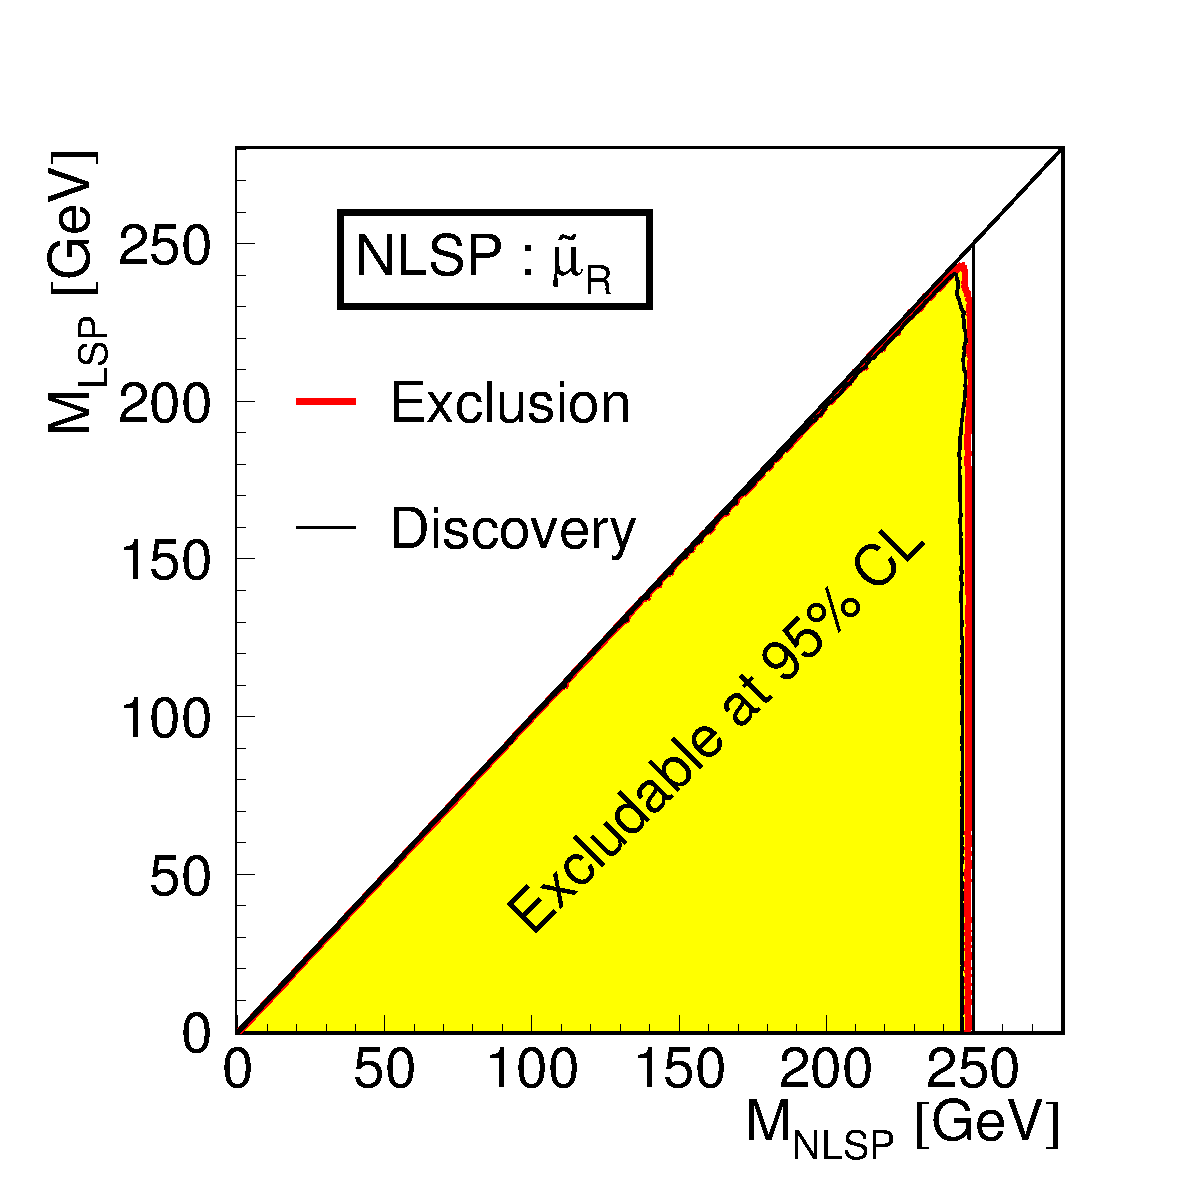
\includegraphics[width=0.35\linewidth]{chapters/figures/smu_nlsp_reach}}
      \hspace{0.1\linewidth}
      \subfigure[]{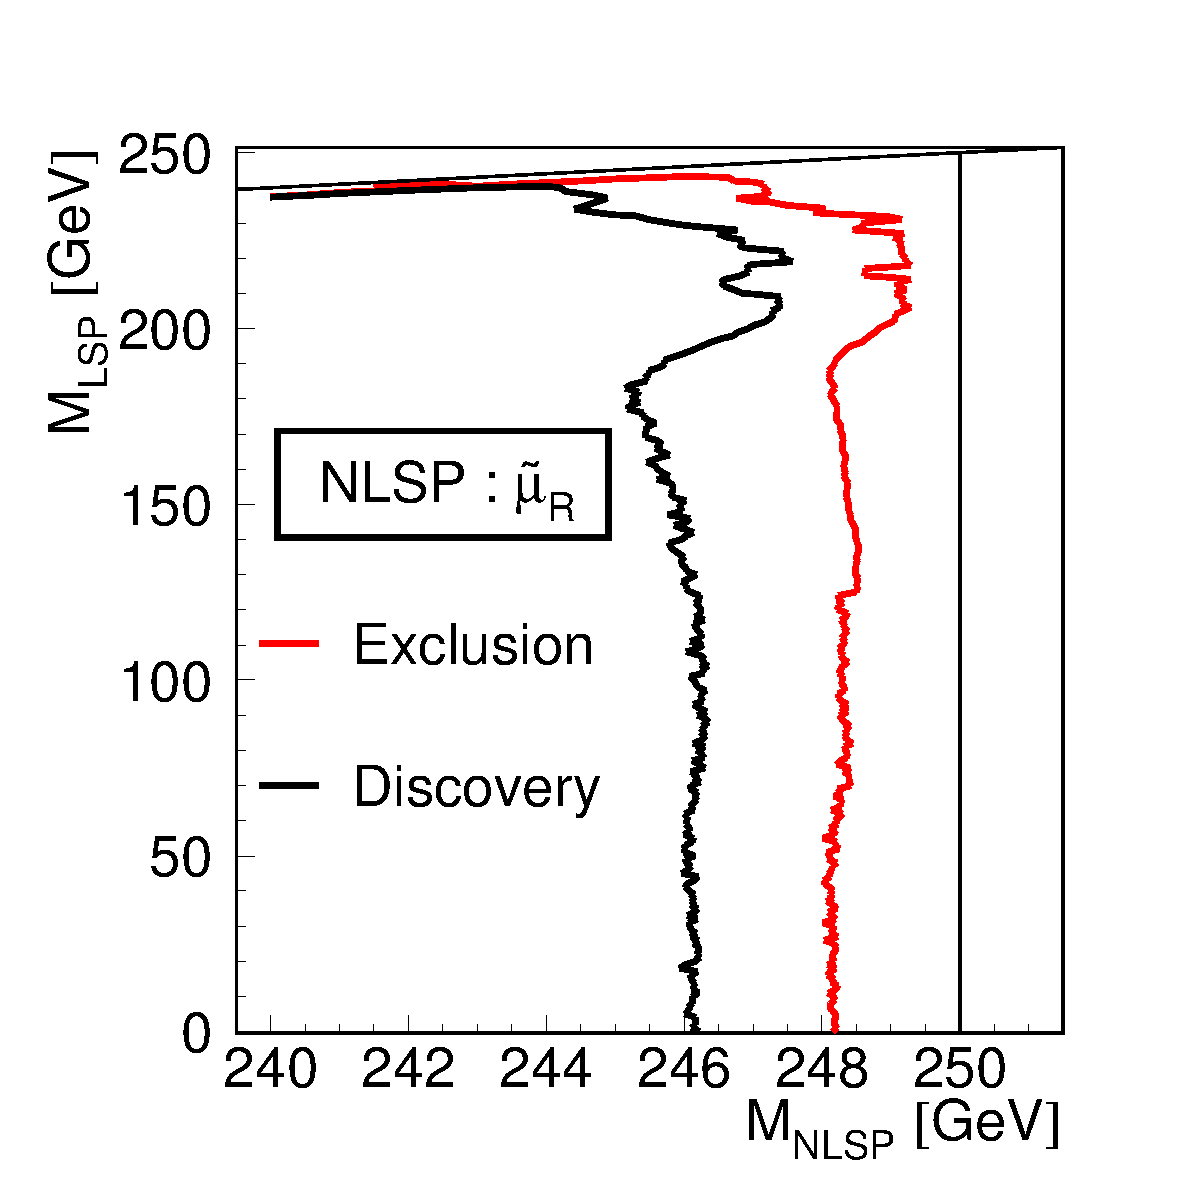
\includegraphics[width=0.35\linewidth]{chapters/figures/smu_nlsp_reach_zoom}}

     \subfigure[]{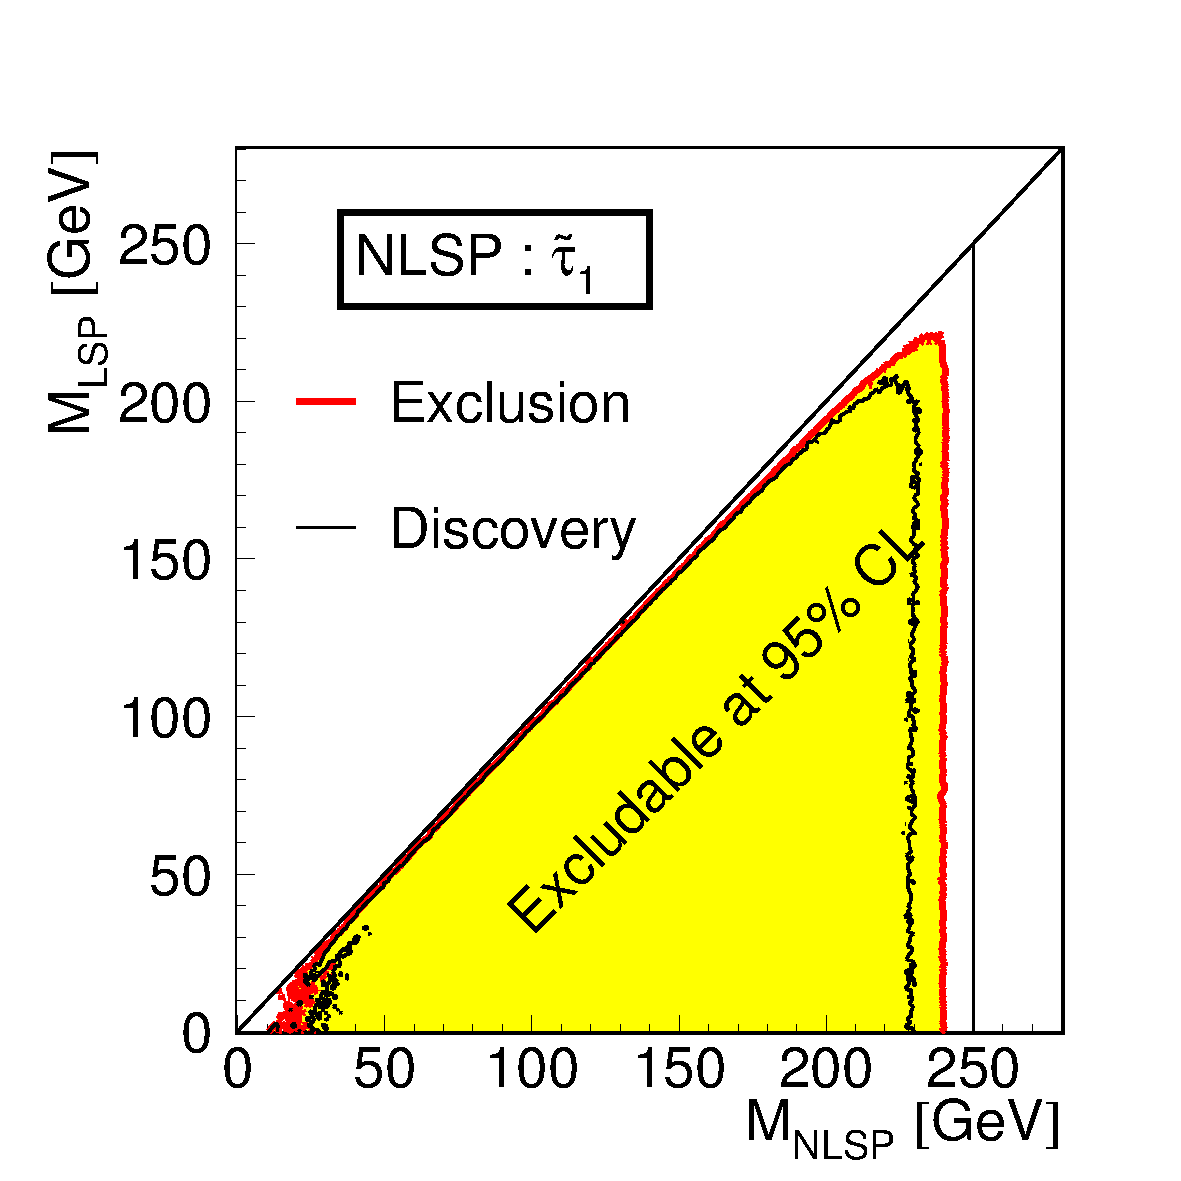
\includegraphics[width=0.35\linewidth]{chapters/figures/stau_nlsp_reach}}
     \hspace{0.1\linewidth}
     \subfigure[]{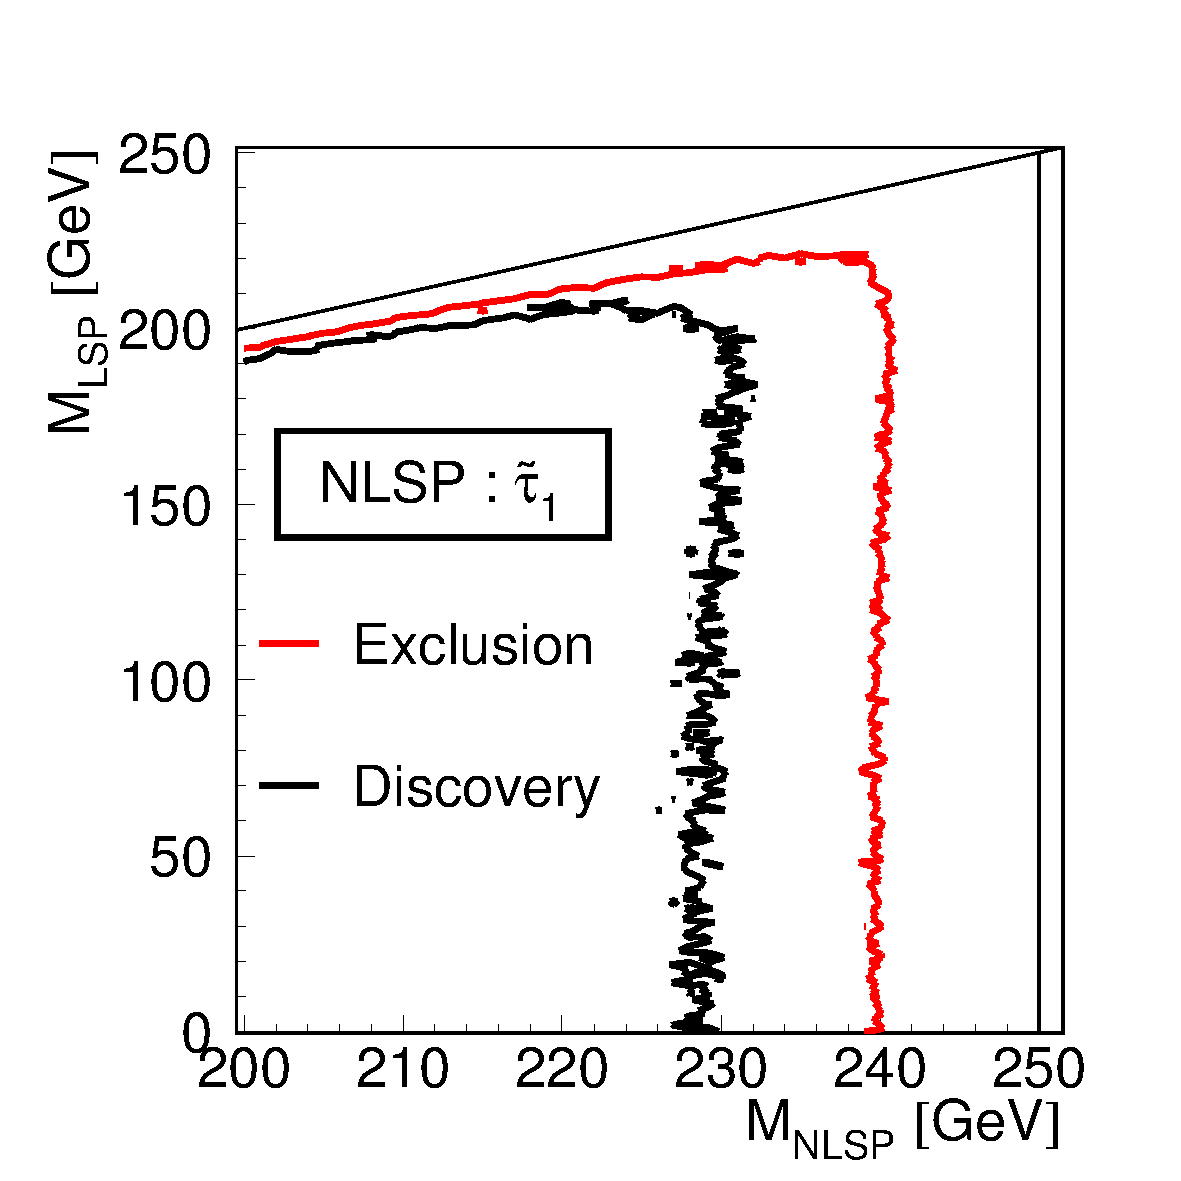
\includegraphics[width=0.35\linewidth]{chapters/figures/stau_nlsp_reach_zoom}}
\caption{ILC discovery reach for a $\smur$ (top) $\stone$ (bottom) 
NLSP for $\int \mathcal{L} \, \mathrm{dt}$ = 
500 fb$^{-1}$ at $\sqrt{s}$ = 500 GeV. 
For the \stone, the mixing angle was chosen to give the lowest
possible production cross-section. (a,c) full scale, (b,d) zoom to last 
few GeV before the
kinematic limit~\cite{Berggren:2013vna}. \label{fig:searches_noloophole1}}
\end{figure*}

In the slepton sector,
smuons and selectrons are excluded
below 95 to 100 GeV, and staus below 87 to 93 GeV. 
Selectrons and
smuons are completely excluded below $M_Z/2$ (from the width of the $Z$),
while staus are excluded below 28 GeV for any mass-difference and
mixing. 
The weaker limit for the staus is due to the fact that
it is possible that the stau mixing is such that it does not couple at
all to the $Z$, 
only to the photon, 
and hence that the constraint from the width of the $Z$ cannot be
applied.
In fact, the limit from the stau at minimal cross-section is the weakest limit on any
NLSP candidate, 
and therefore represents the current absolute exclusion for any MSSM model.

Currently,
LHC has set no limits on processes giving the weakest limits
(sleptons in general, and stau:s in particular)..
In \cite{Aaboud:2017leg,Aad:2014vma,Sirunyan:2018nwe},
it is shown that limits on selectrons and smuons can be set in the best possible case 
- either requiring that not only that both selectrons and smuons 
have the same mass, but also that the left- and right-handed states
are degenerate, or that the mass-difference to the LSP is very large.
No limits at all could be set for stau production.

It can be noted that, except for the chargino,
the LEP limits fall short of the kinematic limit
by 10 to 20 \% even for large mass-differences,
and for small differences by 50 \% or more.
This is due to the fact that the size of the data-sets at the
highest energies were tiny - 500 pb$^{-1}$ at 206 GeV, and
only 33  pb$^{-1}$ at 208 GeV.
This low luminosity is particularly damaging for the sfermions,
because of the slow ($\beta^3$) rise of the cross-section close to threshold.
Also,
the LEP detectors all were triggered,
meaning that in the low mass-difference cases,
either some auxiliary activity was needed to provide
a trigger, 
or only a small fraction of the events - 
those where the detectable SM decay-products happened to be
almost aligned with the direction of the decaying sparticle -
would be registered.
This resulted in a quite low selection efficiency in these cases.
Furthermore,
due to the large size of the beam-spot at LEP,
using impact-parameters as a tool to separate signal
and background was not very effective.
Finally,
the beams at LEP were unpolarised,
which is a particular draw-back when searching for signs
of a chiral theory such as SUSY.

In contrast, the ILC has none of these problems,
as already mentioned,
which means that the ILC at 250 will largely extend the
territory explored by LEP,
much more than the modest increase in energy might suggest at first glance.
In \cite{Berggren:2013vna},
the prospects at the ILC are evaluated.
Two cases were studied in more detail, 
the least and the most challenging ones, 
namely the cases where the NLSP is either the \smur~
or the \stone .
The first case profits from a very clean and well measured
signal,
with no other parameters than the two masses involved,
while the second one has the most difficult signal 
(due to the partly invisible SM system),
and in addition has a further theory parameter,
namely the \stau~ mixing angle.
For both these cases,
the full mass-plane was scanned over a 1-by-1 GeV grid,
using detailed fast simulation.
In the \stone~ case, the mixing-angle was chosen such that the
production cross-section was as small as possible.
The resulting exclusion/discovery reaches are shown in
Figure~\ref{fig:searches_noloophole1}.
One can note that the exclusion limit,
even for the rather modest luminosity used in the study
is only 0.8 (4) \% from the kinematic limit for the \smur (\stone).
The same ratio is expected to hold also for ILC-250.

The area of the mass-plane excludable will increase
by 70 \% to 80 \% at large mass-differences compared to the LEP results.
At the smallest mass-differences,
even larger improvements might be expected,
once dedicated analyses have been performed in this region.

\subsubsection{Sleptons}
\label{subsec:searches_sleptons}
In \cite{Berggren:2015qua} and \cite{Bechtle:2009em}
more in-depth analyses of specific models are presented.
The emphasis in these works is to estimate the precision
with which various parameters can be extracted.
The analyses were done with full simulation at \Ecms = 500 GeV,
but the models studied allows for \selr, \smur. and \stone~production also
at \Ecms = 250 GeV.
\begin{figure*}[]
  \begin{center}
    \subfigure[]{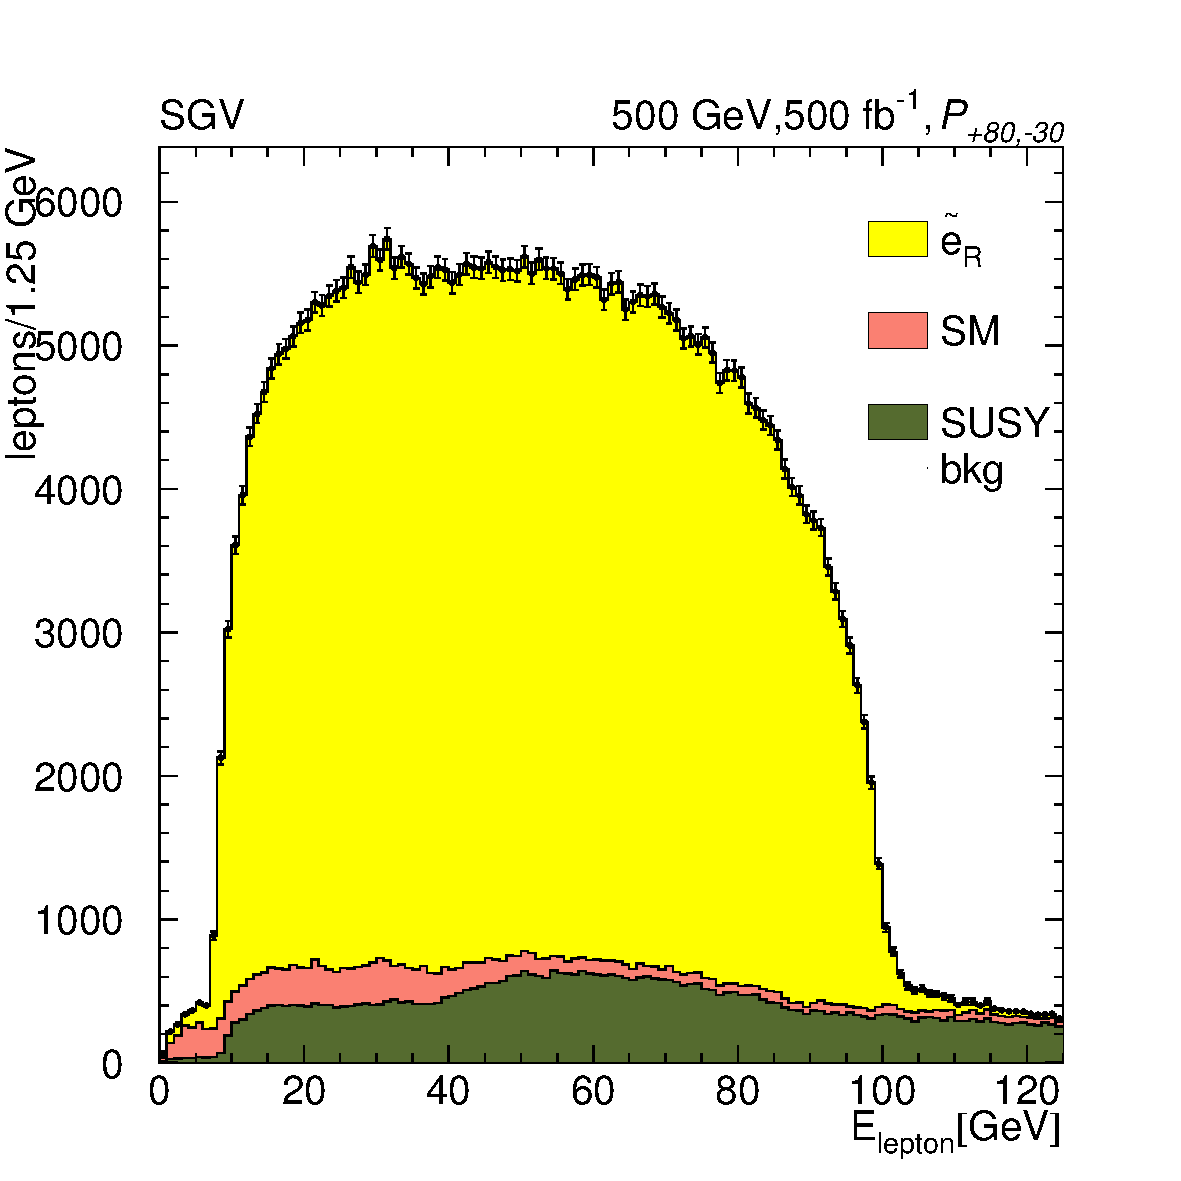
\includegraphics[width=0.3\linewidth] {chapters/figures/serr_tnphs_rl_006_selcuts_skim_whiz6_epj}}
    \hspace{0.01\linewidth}
    \subfigure[]{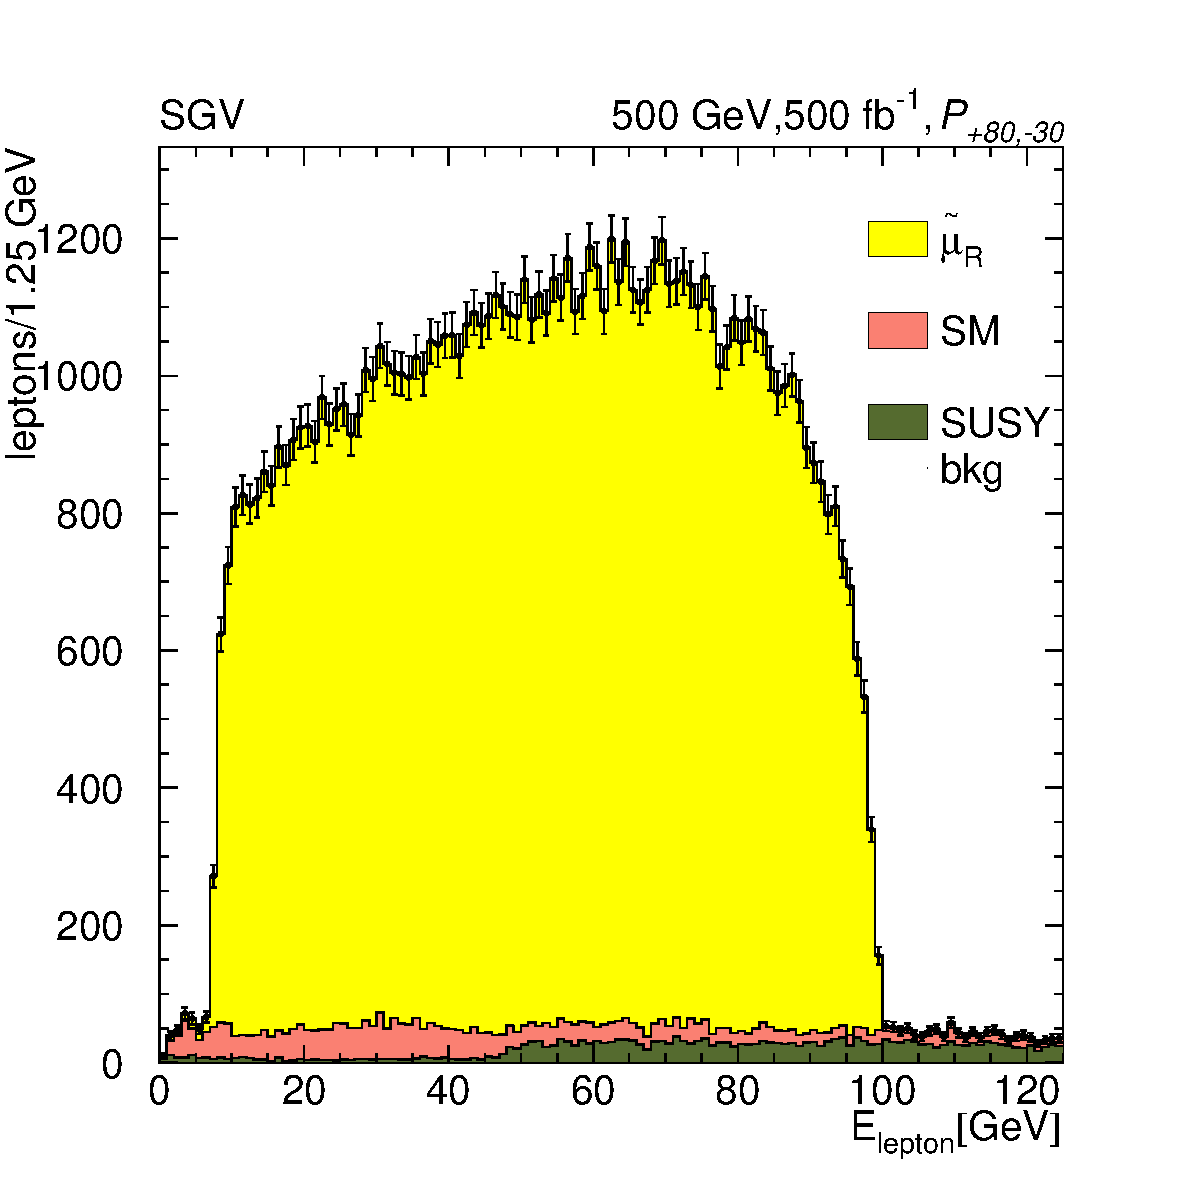
\includegraphics[width=0.3\linewidth] {chapters/figures/smurr_tnphs_rl_006_selcuts_skim_whiz6_epj}}
    \hspace{0.01\linewidth}
    \subfigure[]{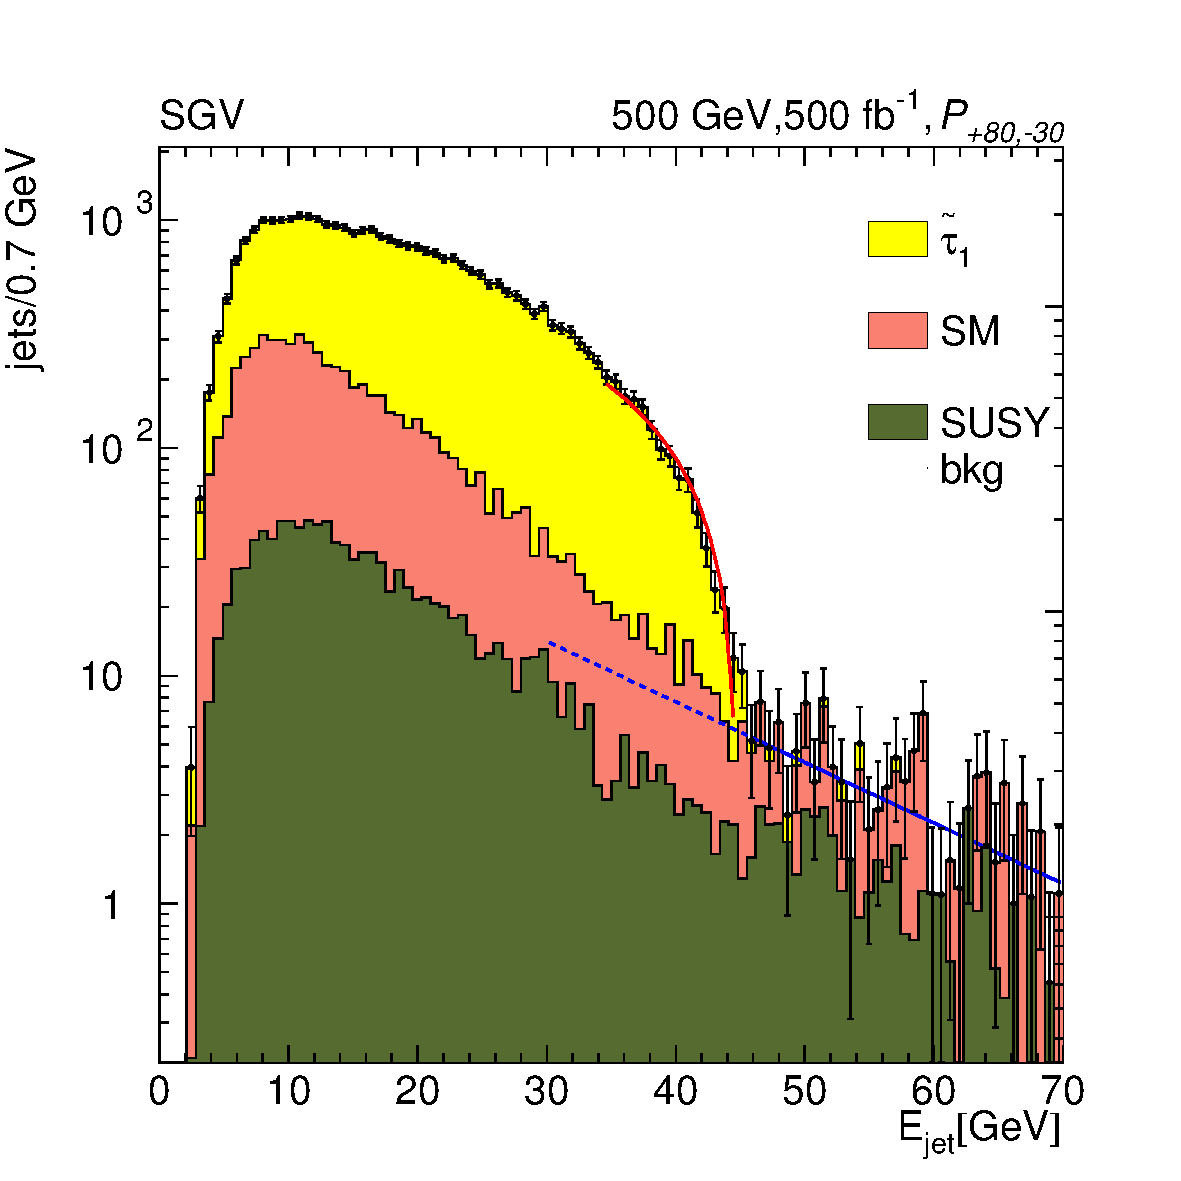
\includegraphics [width=0.3\linewidth]{chapters/figures/stau11-stc-epj-style_wmissch}}
  \end{center}
  \caption{\label{fig:searches_sleptons} Property determination of SUSY  (a) selectron.  (b) muon and 
(c) $\tau$-jet energies in selected di-leptons events
after collecting
500 fb$^{-1}$ of data for beam-polarisation  $\mathcal{P}_{-80,+30}$~\cite{Berggren:2015qua}. }
\end{figure*}
In Figure~\ref{fig:searches_sleptons},
the energy-spectra of the visible decay-products of 
\selr , \smu~and \stone~are shown.
A number of novel techniques were utilised
to extract the relevant edges from the distributions
(the truncated sub-sample method  \cite{Berggren:2015qua},
and finite impulse response method \cite{Caiazza:416980}),
both giving precisions a factor two or more better than
traditional methods.
Once the edges were determined,
applying eq. \ref{eq:searches_genspartendp}
the masses of \selr~ and  \smur~ 
could be estimated with an error of 2~\permil~ and
4~\permil, respectively.
Fitting for a single value of \MXN{1} in these two spectra,
an error of 1.5~\permil~ was obtained.
Using the value of  \MXN{1},
and fitting spectrum in Figure~\ref{fig:searches_sleptons}c for $M_{\stone} $,
the  \stone~mass could be determined to 2~\permil.

Furthermore, 
as can also be seen from eq. \ref{eq:searches_genspartendp},
close to the threshold,
the decay-products become mono-energetic which means
that an almost background-free threshold-scan can be done
at a collider - such as ILC - where \Ecms~ can be freely chosen.
The result of such a scan is shown in Figure~\ref{fig:searches_smuselthreshold}.
The precision of the masses are comparable to those
obtained from the fit to the spectra,
but are independent of \MXN{1}.
In addition,
the fit to the shape of the threshold makes it possible to
exclude the hypothesis that the new states discovered are
fermions,
as can be see by the fits of either $\sigma \propto \beta^3$ (expected for
scalars) or
 $\sigma \propto \beta$ (expected for fermions). 
 
A further measurement possible in these models is the determination of the
polarisation of the $\tau$-lepton from the \stone~ decay.
This is achieved by studying the spectrum of the $\pi$:s in
the $\tau \rightarrow \pi \nu_\tau$ mode, or the ratio of
$E_\pi^\pm$ to $E_\pi^0 + E_\pi^\pm$ in the  $\tau \rightarrow \rho \nu_\tau \rightarrow \pi^\pm \pi^0 \nu_\tau $ mode.
In \cite{Bechtle:2009em} it was found that
the degree of polarisation could be determined to $\sim$ 8 \%.
Also in \cite{Bechtle:2009em},
it was found that the cross-section for \stone~ pair-production could be determined to 4~\%.
The difference in the cross-section when the beam-polarisations are
reversed can be used to determine the \stau~ mixing angle\footnote{The other
possibility to determine the mixing-angle, namely the \stone \sttwo associated production
have not yet been studied in detail},
which together with the determination of $\tau$-polarisation can be used to determine
the size of the chirality-conserving gauagino fraction of the \XN{1} relative to it's
chirality-flipping higgsino fraction.
\begin{figure*}[]
  \begin{center}
    \subfigure[]{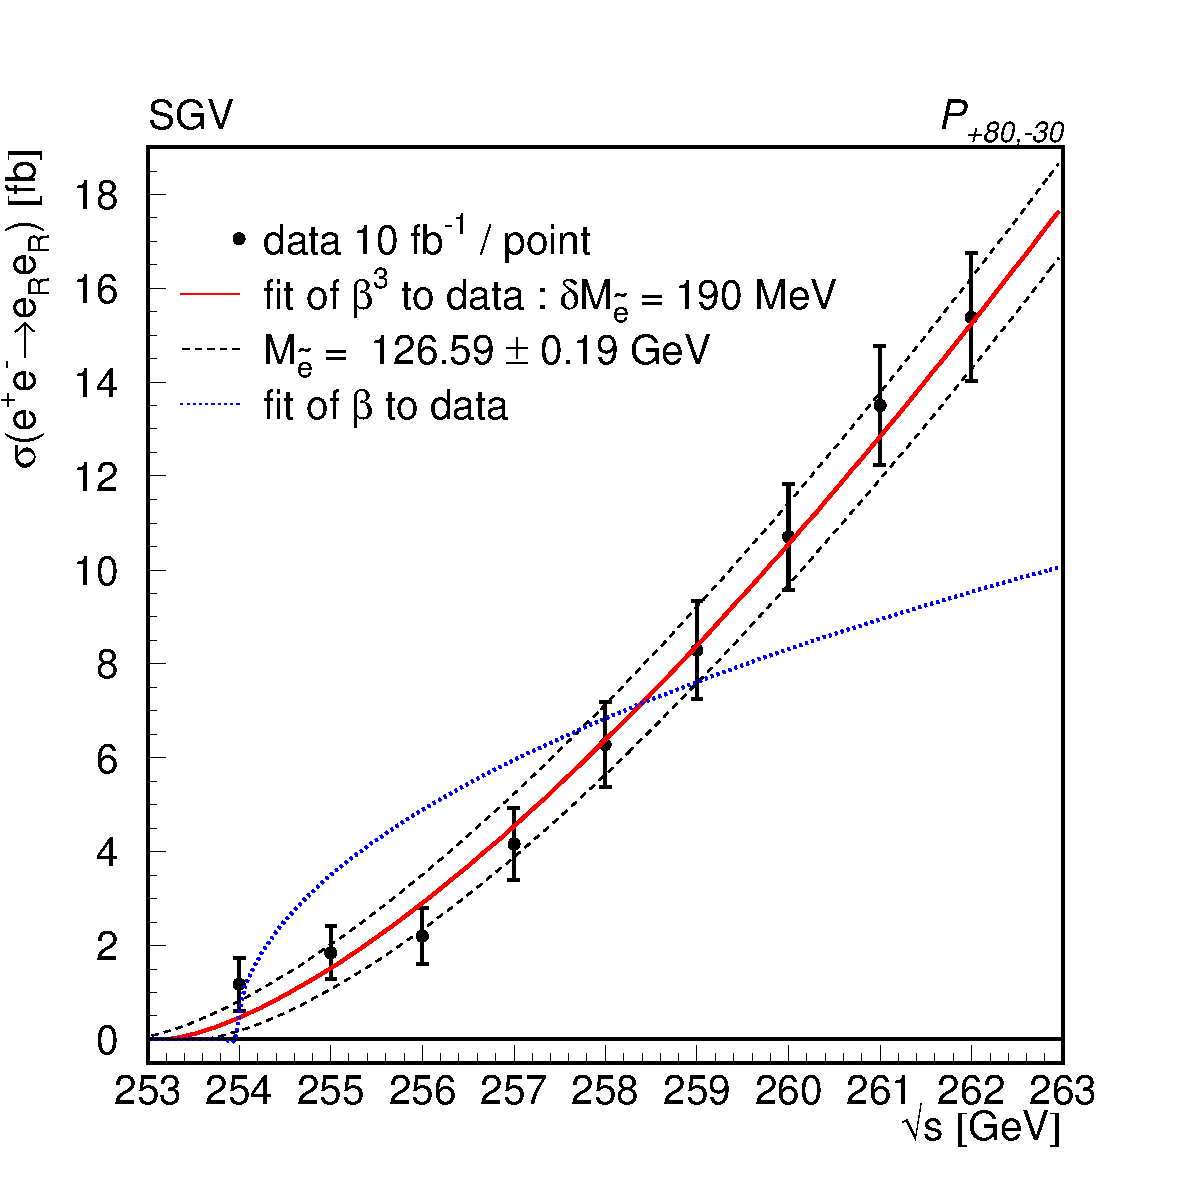
\includegraphics[width=0.3\linewidth]{chapters/figures/STC_selR_threhold-3curves}}
    \hspace{0.01\linewidth}
    \subfigure[]{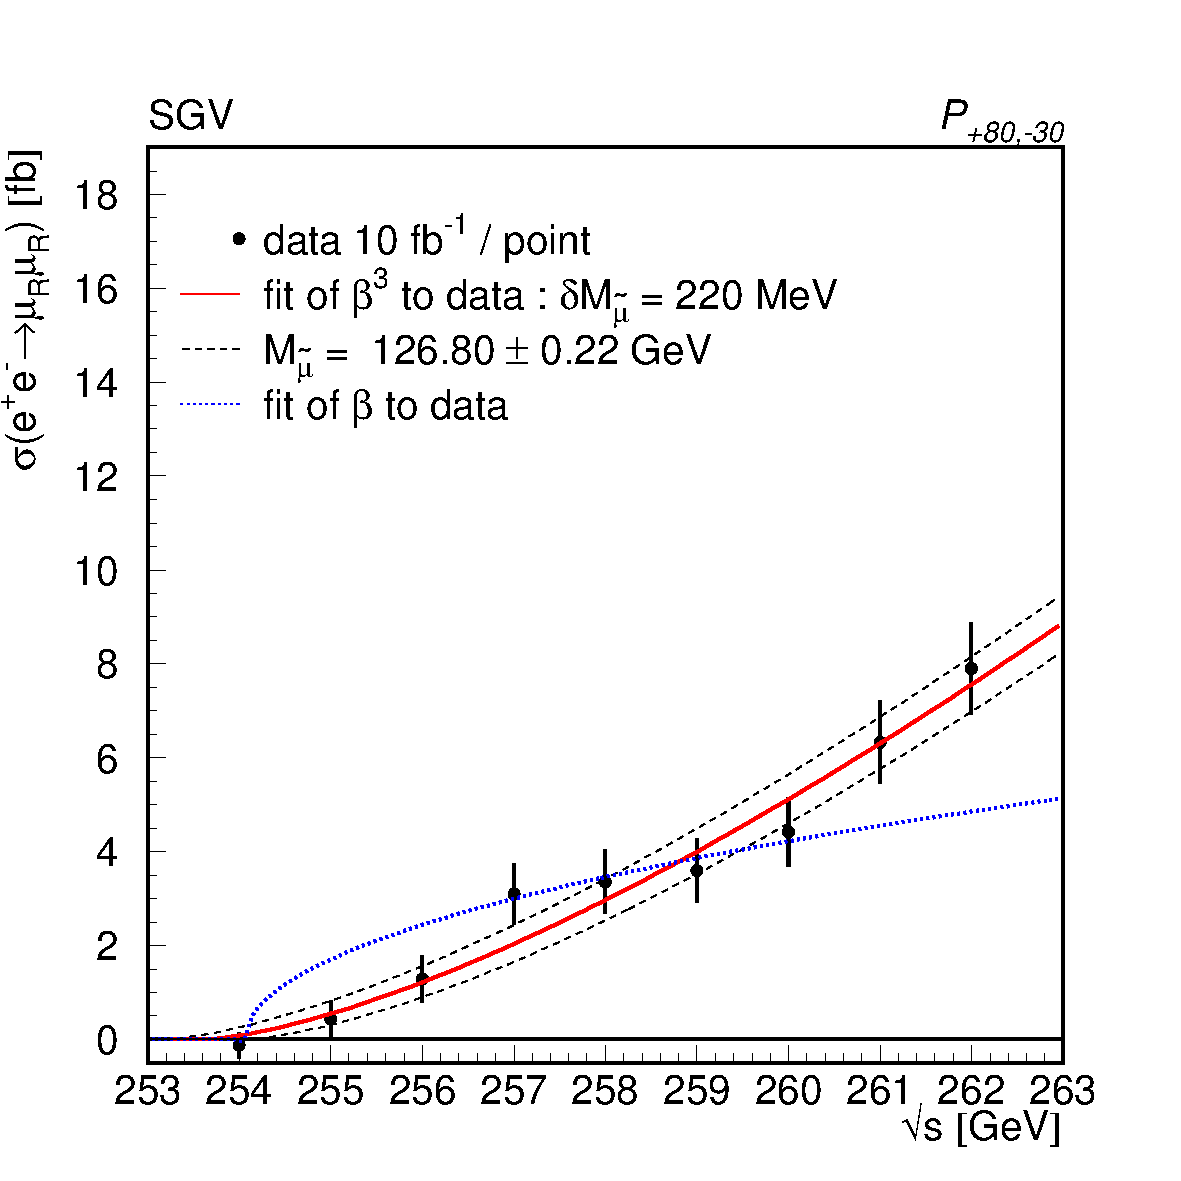
\includegraphics[width=0.3\linewidth]{chapters/figures/STC_smuR_threhold-3curves-uni-scale}}
  \end{center}
  \caption{\label{fig:searches_smuselthreshold} : Scans over the threshold for slepton production
(a) scan of the $\eeto \selr \selr$ threshold  (b)  scan of the $\eeto \smur \smur$ \cite{Berggren:2015qua}. }
\end{figure*}

\subsubsection{Bosinos}
\label{subsec:searches_bosinos}

In \cite{Berggren:2015qua,Berggren:2013vfa,Baer:2016new,Chera:402736}
detailed studies of specific points where a bosino is the NLSP
are presented.
Many different topologies are covered by the analyses,
depending on the mass-difference.
The bosinos might decay to on-shell $Z$ or $W$ bosons,
undergo three-body decays (mediated by virtual
$Z$ or $W$ bosons), or decay radiatively.
In addition,
mixing in the bosino-sector will yield relations between the masses
of $\XN{2}$, $\XPM{1}$ and the LSP, relations that are different
for different models.
The same is true for the production cross-sections,
in particular the relation between $\XN{2}\XN{2}$
pair-production and
$\XN{1}\XN{2}$ associated production.
Also assumed relations at the high scale have implications on
the phenomenology at the EW-scale,
in particular on how large the LSP-NLSP mass difference can be.
For bosino production it is therefore needed to study
various cases in detail,
and avoid assumptions on other related processes.
The LEP experiments all carried out a comprehensive
search for a $\XPM{1}$ NLSP which were combined in \cite{LEPSUSYWG/02-04.1}.
For the   $\XN{2}$ NLSP case,
as mentioned above,
only cross-section limits can be given,
if no assumptions on the model is done.
Such limits were given by the experiments \cite{Abdallah:2003xe,Acciarri:1999km,Abbiendi:2003sc}.
% No ALEPH final say ?!

At LHC, the reach of the search for the non-coloured bosinos
can be quite large, but always with strong model assumptions.
Even so, the limits tend to disappear for low mass-differences,
and are largely absent in the region allowed if GUT-scale unification
of the bino and wino mass-parameters ($M_1$ and $M_2$) is assumed
\cite{Aaboud:2018jiw,Aaboud:2017leg,Sirunyan:2018ubx}.

Once again, the conditions at the ILC will allow to extend the
model-independent LEP limits to higher masses.
Because the $\XPM{1}$ cross-section is quite large, and has
a sharp ($\propto \beta$) threshold dependence,
the increase in reach at ILC-250 with respect to LEP is
not as large as it is for the sfermions: already LEP could
exclude  an $\XPM{1}$ NLSP to only a few GeV below the kinematic limit
and at all mass-differences.
Nevertheless,
the limit/discovery potential of ILC-250 is sizeable
compared to current and future LHC limits,
in particular as the LHC limits for bosinos suffer
more from model-dependence than the sfermion ones.
The ILC potential
becomes very important at a future energy-upgrade. 

This is illustrated by a specific example in figure~\ref{fig:searches_bosinoexcl}, 
which shows the current limits in the $\MXN{1}$ - $\MXC{1}$ 
plane from ATLAS~\cite{Aad:2014vma}, together with the
projected discovery reach at 14 TeV with $\int \mathcal{L} \, \mathrm{dt}$ = 3000 
fb$^{-1}$ \cite{ATL-PHYS-PUB-2018-048}
%ATLAS:2013hta}.
Here it is assumed that  $\MXN{2}=\MXC{1}$, that $\XPM{1}$ and $\XN{2}$ are 
pure Winos, and that Br($\widetilde{\chi}\rightarrow W^{(*)}/Z^{(*)}\XN{1}$)
=1
\footnote{Note that the more difficult case $\widetilde{\chi}\rightarrow h^{(*)}\XN{1}$ is 
not considered.}.
The brown-shaded area indicates the corresponding limit from LEP 
\cite{Heister:2002mn,Abdallah:2003xe,Abbiendi:2002vz},
which assumes only  $\XPM{1}$ pair production, with no assumption on the decay mode,
nor the nature of the $\XPM{1}$.
The expected limits for the ILC at $\sqrt{s}=500$ or $1000$\,GeV are also shown 
with the same 
assumptions as for the LEP exclusion.
As can be seen from the (loophole) region not covered by the LHC, there is a large
discovery potential for the ILC, even after the high luminosity LHC data has been 
fully exploited.

\begin{figure*}[]
   \centering
      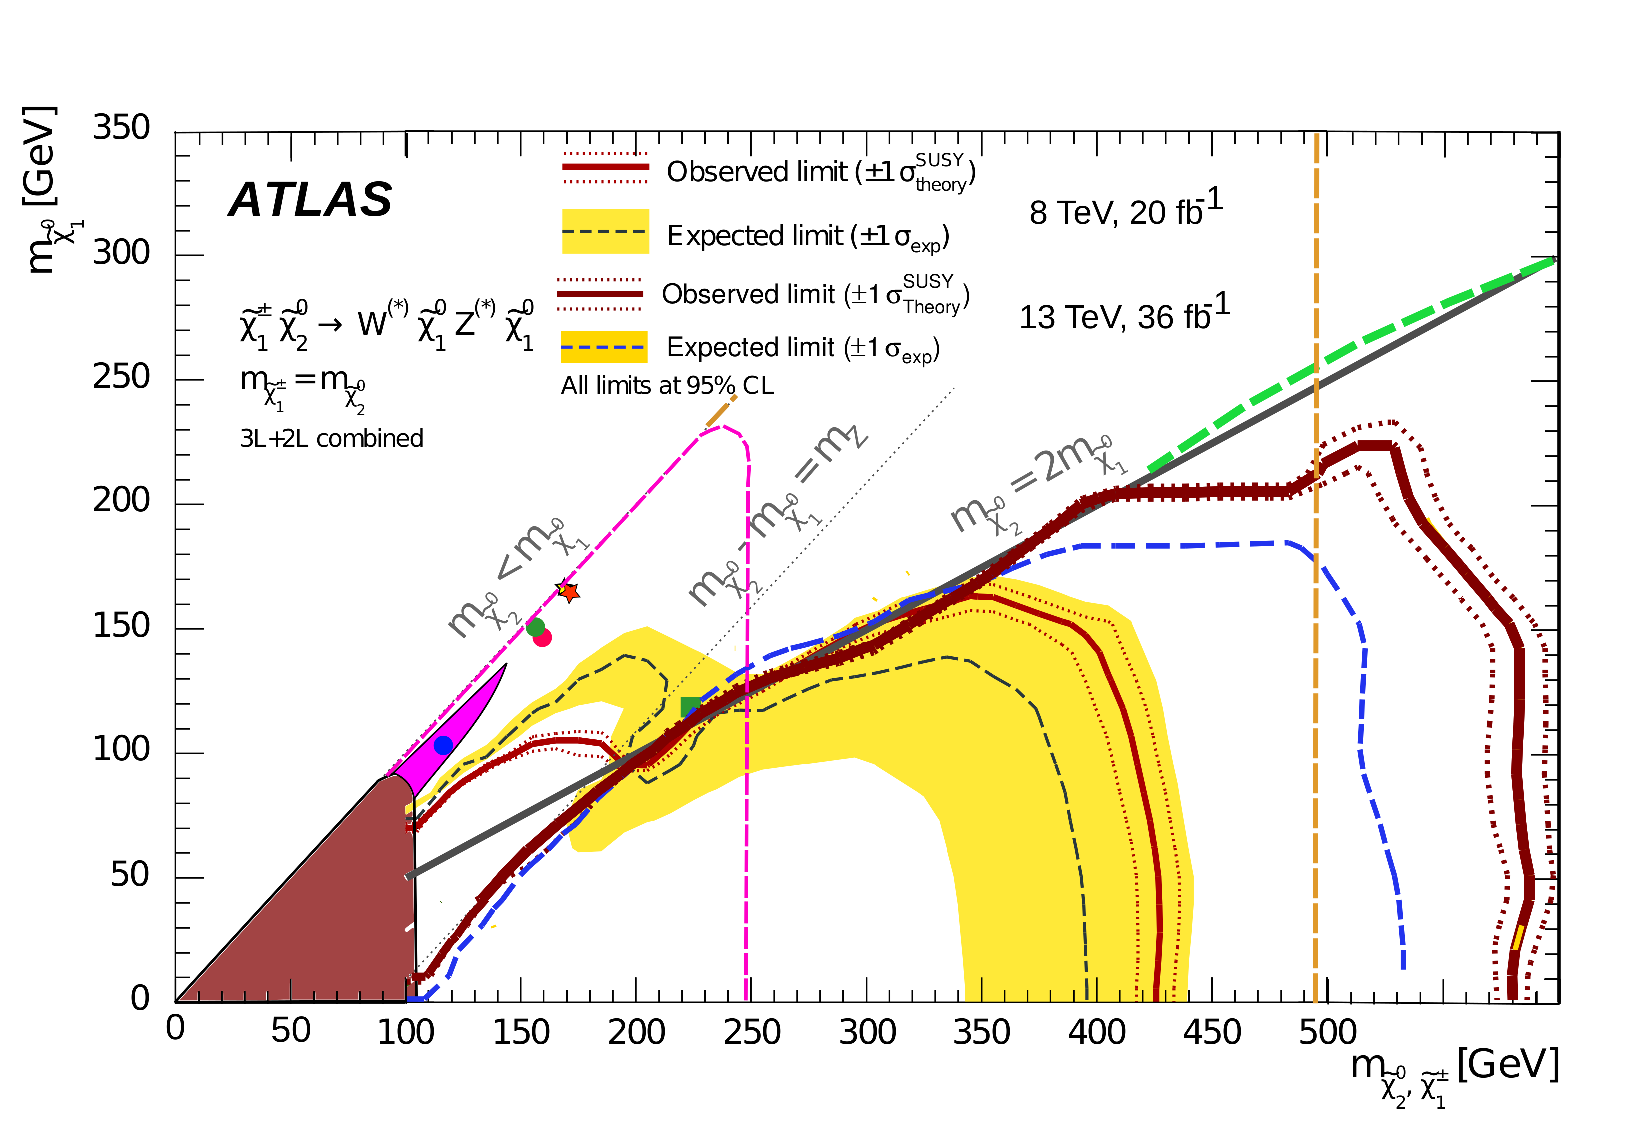
\includegraphics[width=0.5\linewidth]{chapters/figures/fig_08d_w_lep_w_lhc_lodm_w_bmark_w_hlproj_w500_w1000}
%%%.eps.gzfig_07b_w_lep_lhc14_n_hilum_ilc500_ilc1000_proc}
\caption{Discovery or exclusion regions in the $M_{NLSP} - M_{LSP}$ plane
  for a $\XPM{1}$ or $\XN{2}$ NLSP. Solid brown area: LEP exclusion;
  Solid red and dashed grey/blue lines: ATLAS exclusion (observed and expected),
  for the 8 TeV data (thinner lines) and the 13 TeV data (thicker lines).
  Dashed green line: ATLAS 14 TeV discovery projections for $\int \mathcal{L} \, \mathrm{dt}$ = 3000 fb$^{-1}$;
  Dashed magenta (orange) lines: ILC discovery expectation for $E_{CMS}$ = 500 (1000) GeV;
  Solid black line: below line, no GUT scale gaugino mass unification.
  The symbols indicate the positions in the mass-plane of the analyses mentioned in the text.
  The magenta solid area is the ATLAS low $\Delta(M)$ search at 13 TeV, which however is within a different model.
%% For further details, see text. 
 \label{fig:searches_bosinoexcl}}
\end{figure*}

\subsubsection{Small mass differences}
\label{subsec:searches_lowdm}
The case with Antler topologies with small mass-differences
is particularly interesting for ILC-250.
Partly because the experimental limits from LEP are much weaker then
for high mass differences,
and largely absent at LHC,
but also for theoretical reasons.

One reason to particularly search for SUSY with small
mass-differences is the possibility that the LSP is the (full) explanation
for Dark Matter:
Over a large region of SUSY parameter space, co-annihilation with the NLSP
is an attractive mechanism which acts to reduce the relic density of the LSP to its
cosmologically observed value~\cite{deVries:2015hva}. 
An example of such a model is the one presented in~\cite{Berggren:2015qua} and
discussed in the previous section.
In this model,
the NLSP is the \stone,
with a mass 10 GeV above the LSP.
Co-annihilation requires
a small mass difference between the NLSP and the LSP in order to be effective,
and thus the expected value of the relic density depends strongly on the exact
masses and mixings of the involved particles, requiring measurements at the permille and
percent-level, respectively.
This is discussed in~\cite{Lehtinen:415433}, 
where also a detailed analysis of the relic-density determination that
the measurements presented in~\cite{Berggren:2015qua} would imply.
Figure~\ref{fig:searches_STC10omega}a shows the precision
of the fitted relic density relative to the model value.
In the figure, 
the model value was chosen to be
the central value determined from cosmology using the observations 
of {\sc planck}~\cite{Ade:2015xua}.
It was also verified the other model-values were faithfully reproduced
by the fit, see Figure~\ref{fig:searches_STC10omega}b.
\begin{figure*}[]
   \centering
      \subfigure[]{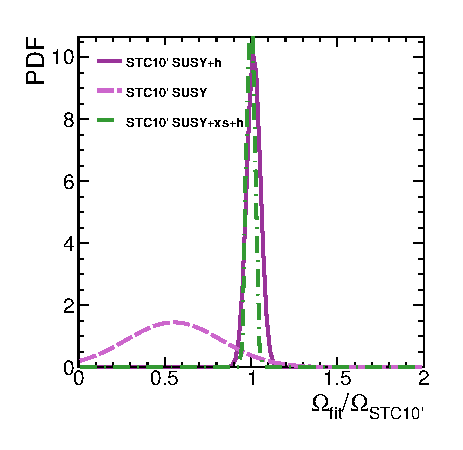
\includegraphics[width=0.35\linewidth]{chapters/figures/suvi_omega_6_31}}
      \hspace{0.1\linewidth}
      \subfigure[]{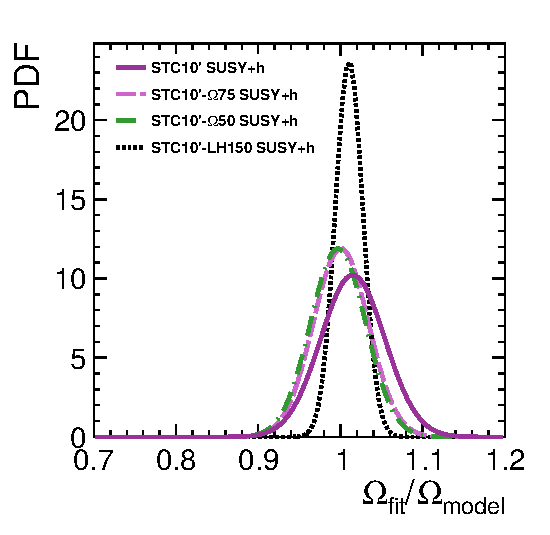
\includegraphics[width=0.35\linewidth]{chapters/figures/suvi_omega_6_40}}
\caption{ (a) Comparison  of  relic   density  fitted to  the   measurements of the SUSY model
to the model value, with or without using input from ILC higgs-measurements and with, in addition, using 
measured cross-sections. (b) Comparison between fitted and model value, when the model value was by hand modified as indicated.
From~\cite{Lehtinen:415433}. \label{fig:searches_STC10omega}}
\end{figure*}


A second, different, reason to search for such low mass-difference
processes, applying to SUSY
is that they tend to occur in many possible SUSY scenarios:
As shown in Figure~\ref{fig:searches_tomohikoscan},
because of the mass-relations between different bosinos in the Wino- and
Higgsino-sectors,
the second lightest bosino will be close in mass to the LSP,
if the latter is dominantly Wino or Higgsino.
Only in the case of a large admixture of Bino in the LSP
can the mass-difference be arbitrarily large.
Furthermore, 
{\it if} GUT-scale unification of  the Bino and Wino mass 
parameters $M_1$ and $M_2$ holds,
the next-to-lightest bosino {\it cannot} be heavier the twice the LSP mass.
\begin{figure*}[]
  \begin{center}
    \subfigure[]{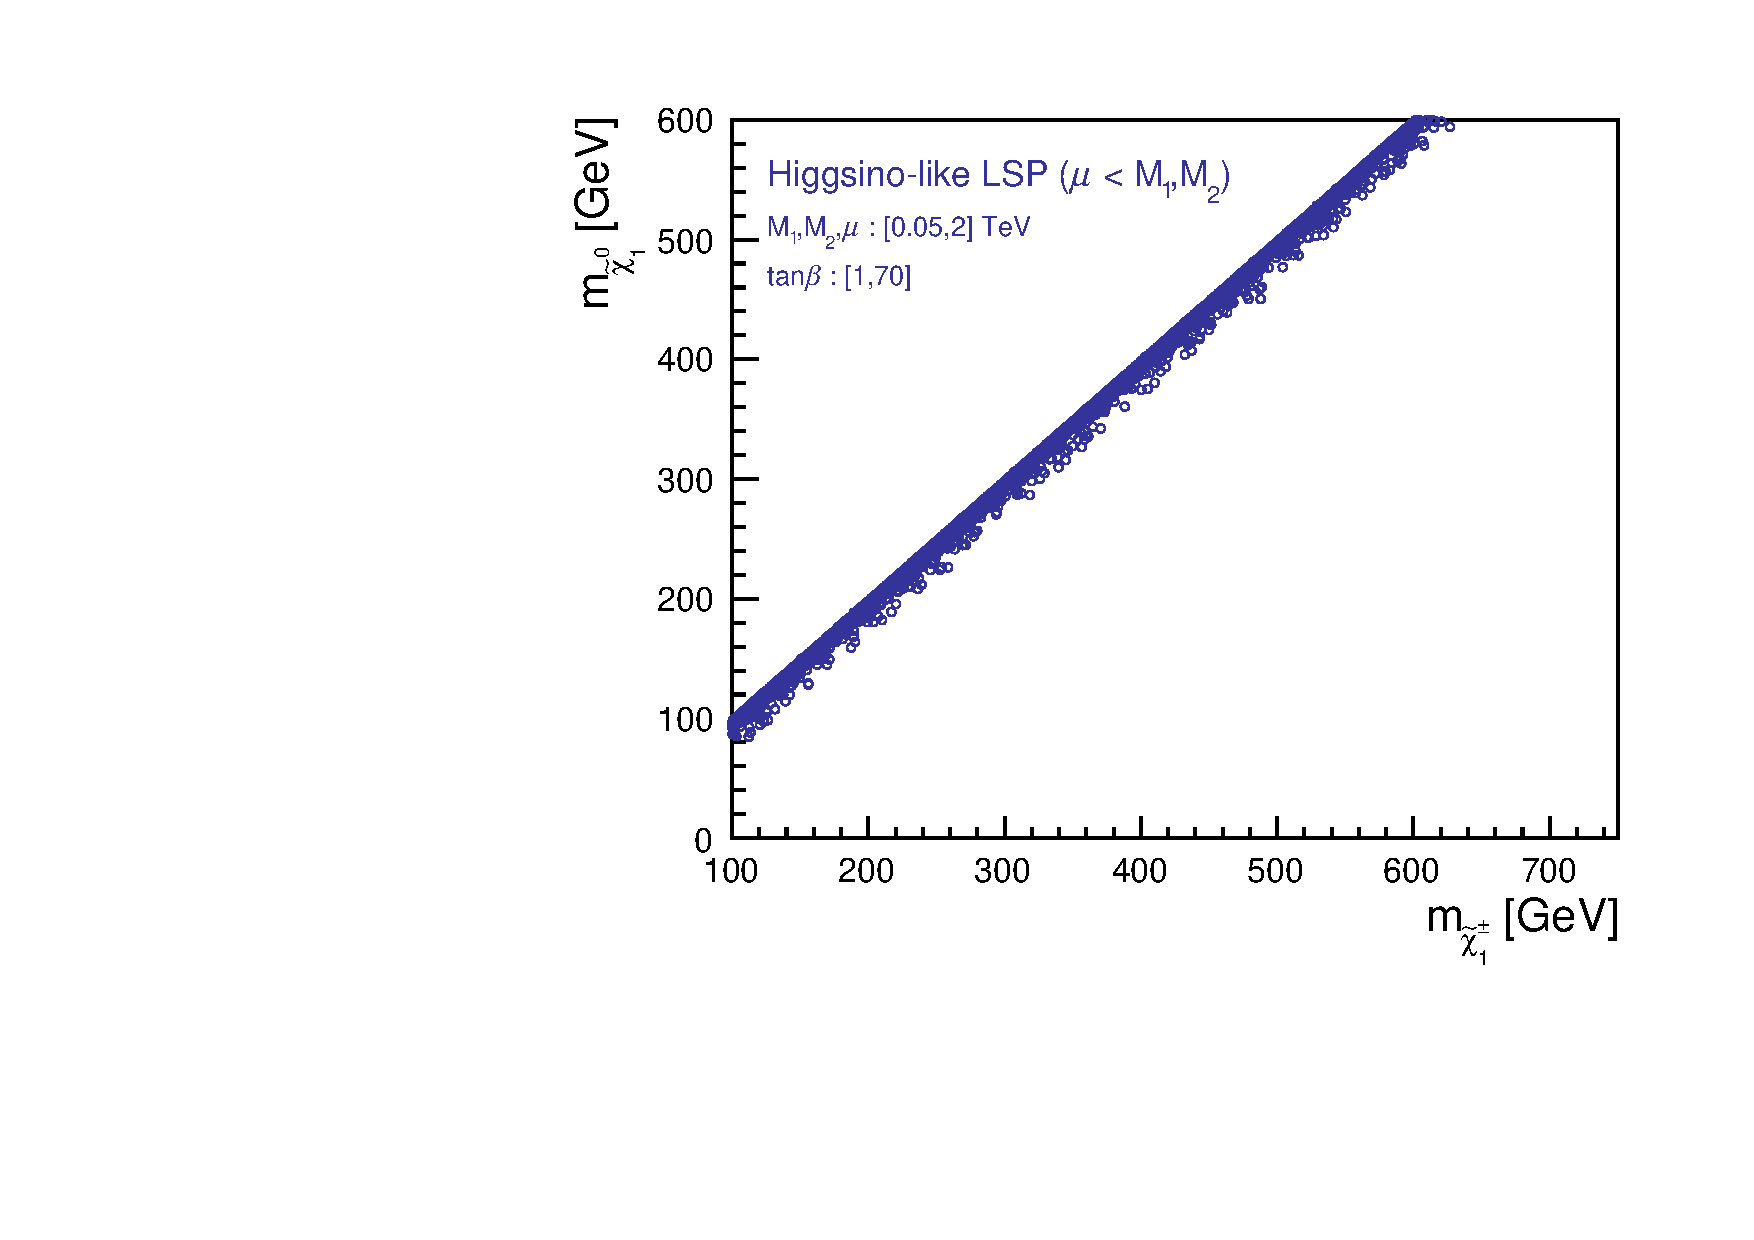
\includegraphics[width=0.3\linewidth] {chapters/figures/higgsino-like2}}
    %\hspace{0.05\linewidth}
    \subfigure[]{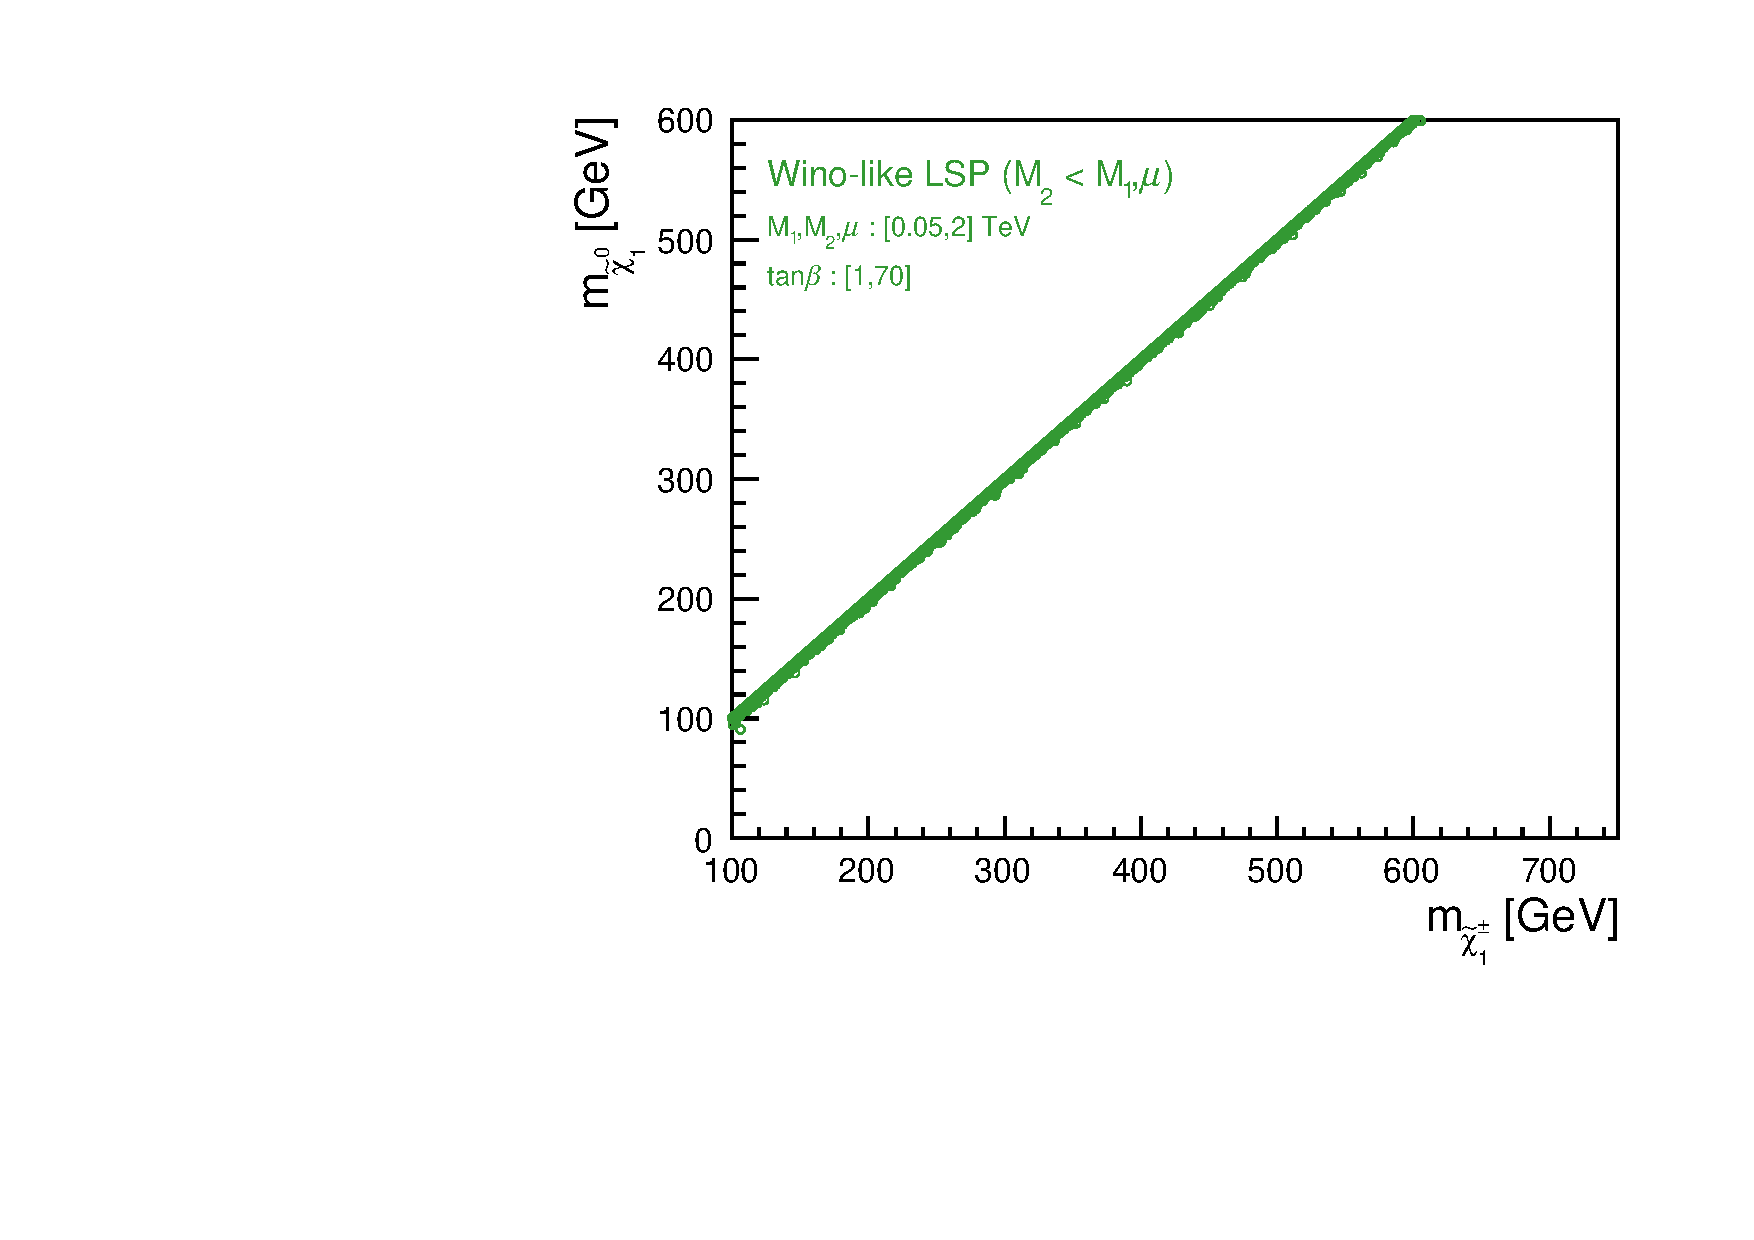
\includegraphics[width=0.3\linewidth] {chapters/figures/wino-like2}}
    %\hspace{0.05\linewidth}
    \subfigure[]{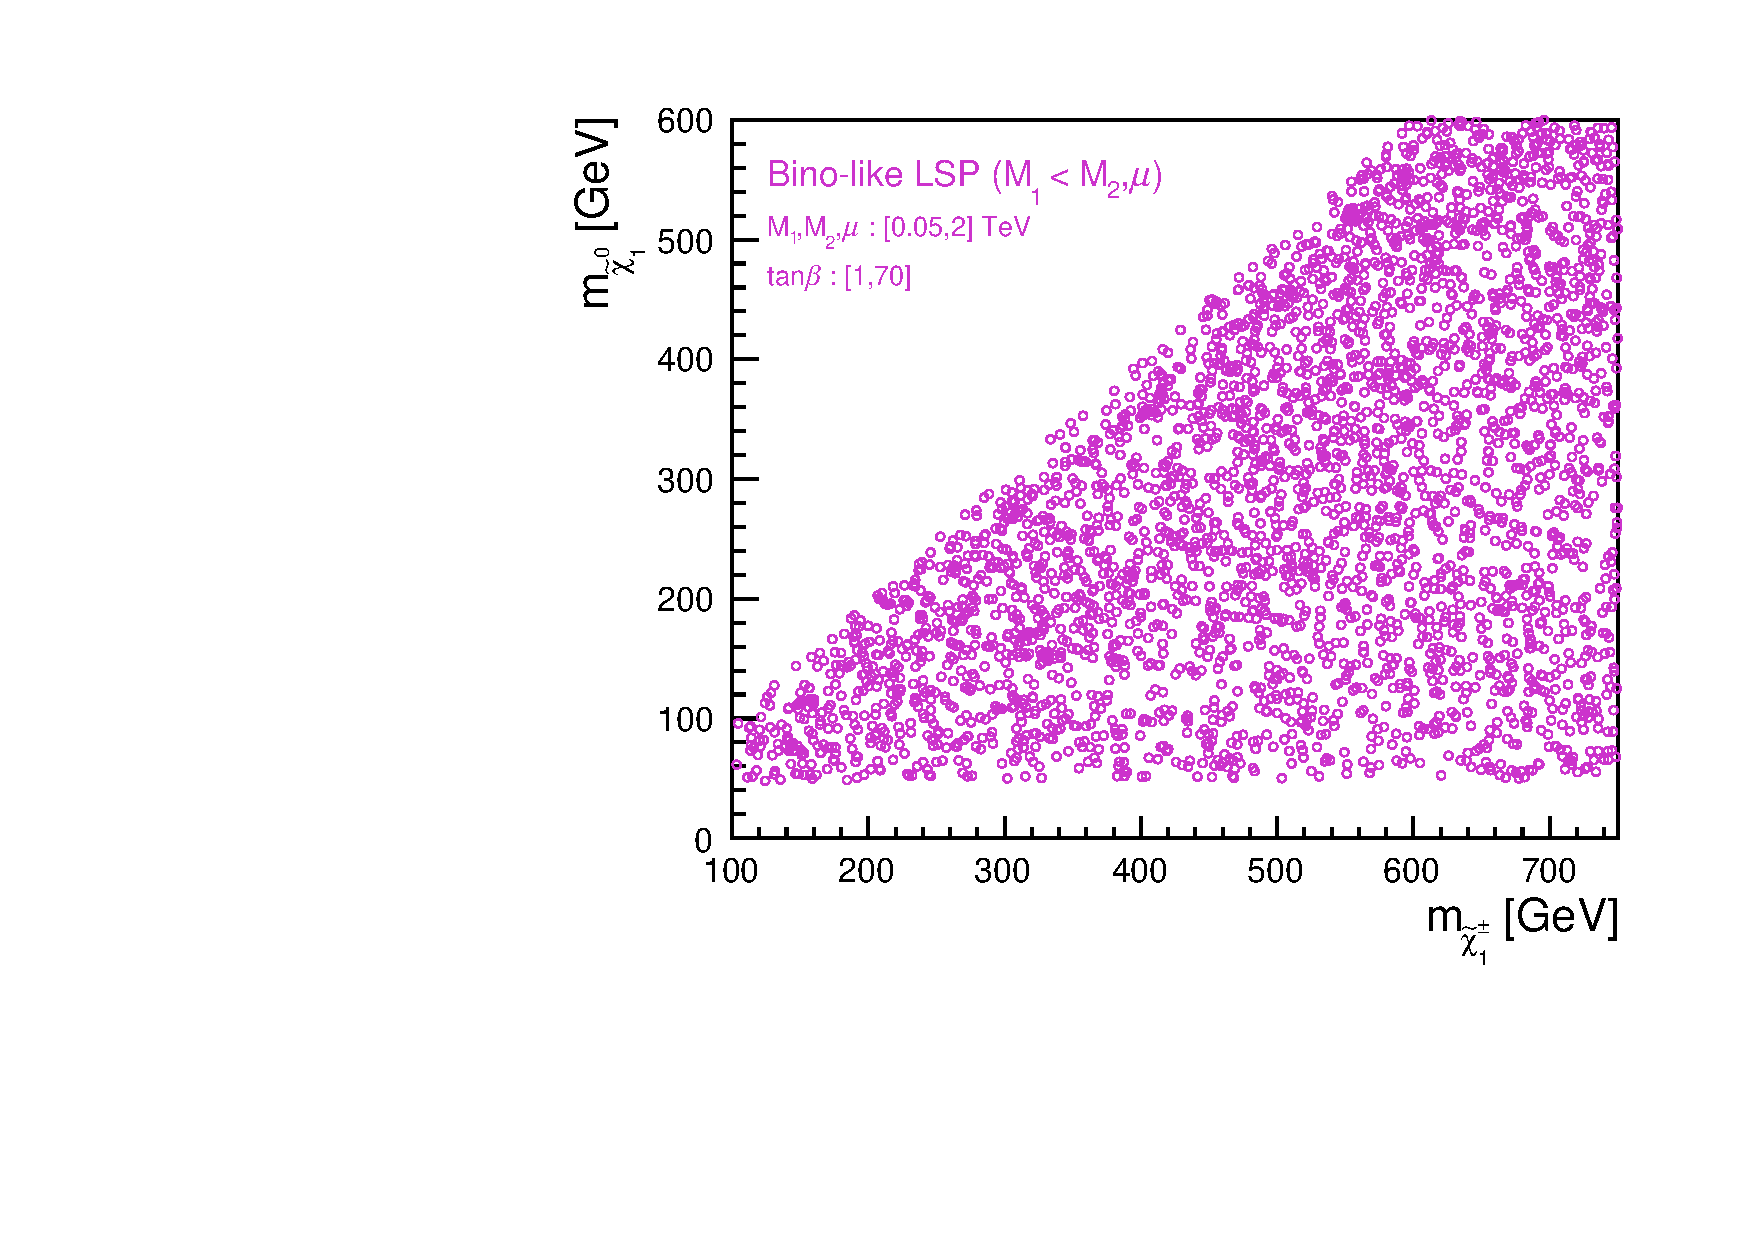
\includegraphics[width=0.3\linewidth] {chapters/figures/bino-like2}}
  \end{center}
  \caption{\label{fig:searches_tomohikoscan} \MXN{1} vs \MXC{1} when scanning over the bosino parameters
$M_1 , M_2, \tan{\beta}$ and $\mu$. (a) Higgsino-like LSP ($\mu < M_1 , M_2$), 
(b)  Wino-like LSP ($M_2 < \mu , M_1$), (c) Bino-like LSP ($M_1 < \mu , M_2$). }
\end{figure*}

In fact, 
light higgsinos are a fundamental requirement 
of natural SUSY models.
The generic formula relating $M_Z$ to SUSY parameters reads
~\cite{Bae:2014yta}:
\begin{align}
\frac{m_Z^2}{2} =& \frac{(m_{H_d}^2+\Sigma_d^d)-(m_{H_u}^2+\Sigma_u^u)\tan^2\beta}{(\tan^2\beta -1)}
-\mu^2\simeq -m_{H_u}^2-\mu^2
\label{eq:searches_mzs}
\end{align}
To avoid unnatural fine-tuning between the terms on the right-hand side in
this expression, each term should individually be of the order of the left-hand side,
i.e.  $M^2_Z$,
and in particular $\mu$ should be as close as possible to $M_Z$.
This leads to a dominantly higgsino LSP and that
also $\XN{2}$ and $\XPM{1}$ are mainly higgsino.
Mass differences within the higgsino sector are small, 
typically  below $20$\,GeV,
depending on the values of the other SUSY parameters, 
in particular on $M_1$ and $M_2$.
The other SUSY particles can be more heavy:
top squarks may range up to $\sim 3$ TeV and gluinos 
up to $\sim 4$ TeV with little cost to naturalness~\cite{Bae:2014yta}. 
Such heavy top squarks and gluinos may well lie beyond the reach of even HL-LHC.

In the clean environment of the ILC, the soft visible
decay products of $\XN{2}$ and $\XPM{1}$ can be easily detected 
--- without any need to rely on large-mass-gap decays
of heavier particles. 
The ILC capabilities 
have been studied in detector simulations performed for different 
benchmark points with mass 
differences ranging from $770$\,MeV~\cite{Berggren:2013vfa}
to $20$\,GeV~\cite{Baer:2016new}. 
\iffalse
{\color{red} Can one make point 5 fit in here somehow. Then the Atlas+LEP+ILC plot
could go here somehow. Or a new subsection on Antler's to bosons? }
\fi
Two examples of the striking signals and the extraction of 
kinematic endpoints are given in Fig.~\ref{fig:searches_higgsinos}. 
The resulting precisions on masses and polarised 
cross sections reach the percent level even in the experimentally most difficult 
cases and allow to determine other SUSY parameters.
They will also play an important role in unveiling the nature of dark matter: 
in this case with the result that the LSP only contributes a small fraction of the 
total abundance. Such a situation might call for additional, non-WIMP constituents of 
dark matter such as axions:

\begin{figure*}[]
  \begin{center}
    \subfigure[]{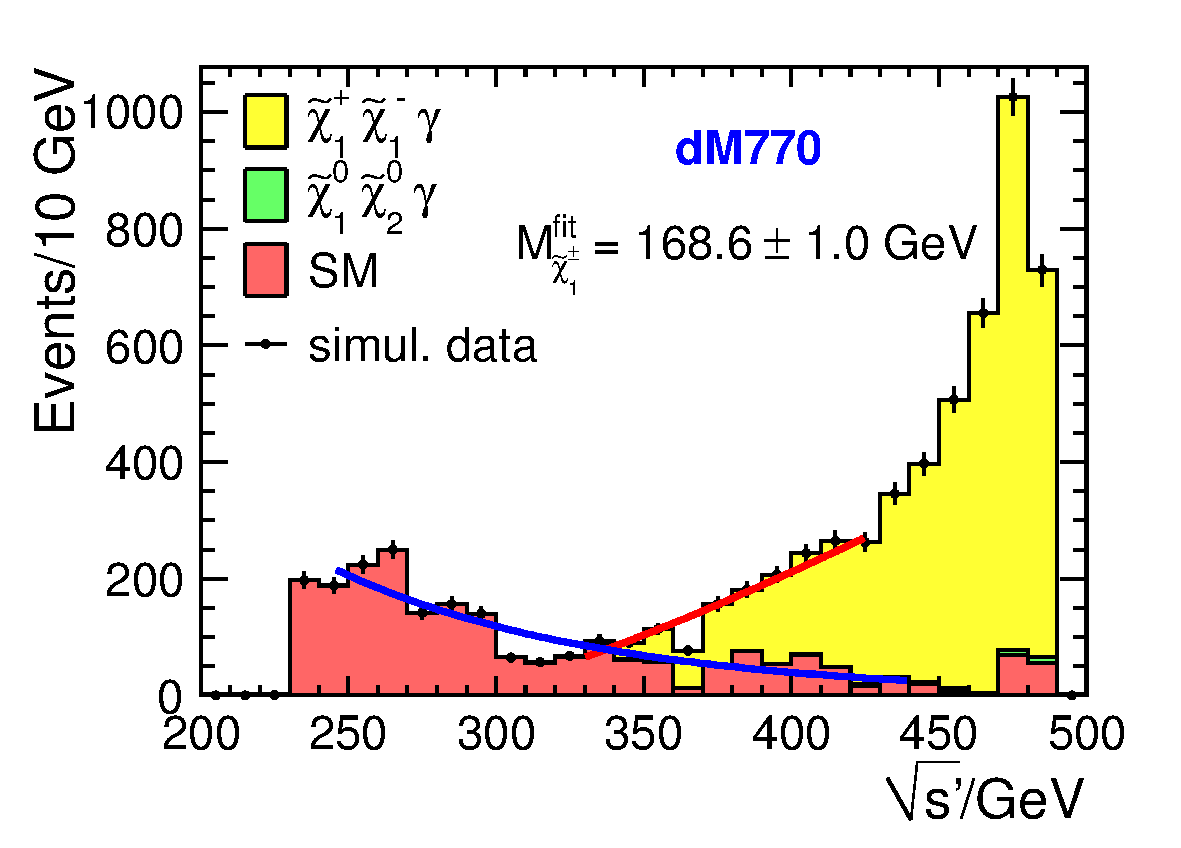
\includegraphics[width=0.45\linewidth] {chapters/figures/MrecoilC_mh127}}
    \hspace{0.05\linewidth}
    \subfigure[]{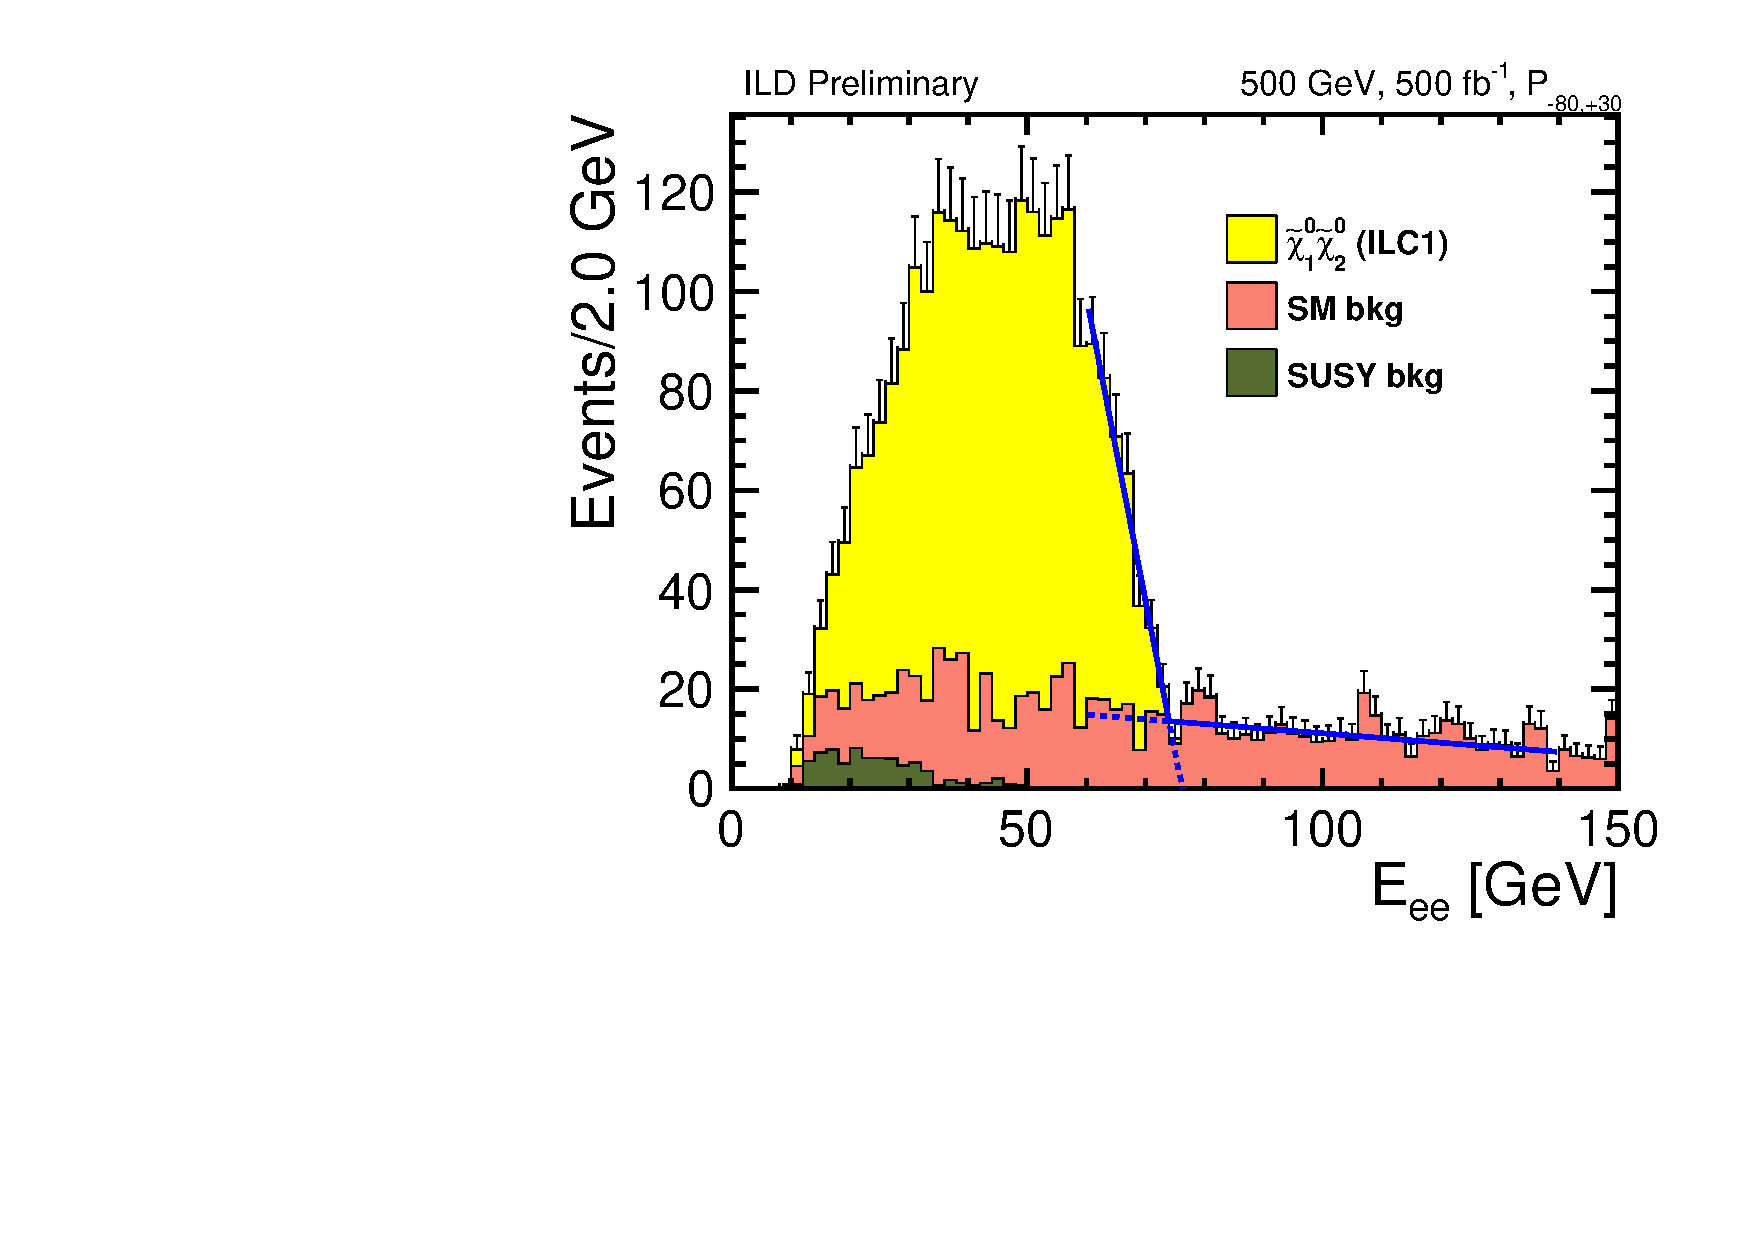
\includegraphics [width=0.45\linewidth]{chapters/figures/EdleeL.pdf}}
  \end{center}
  \caption{\label{fig:searches_higgsinos} Higgsino mass determination for (a) the charged higgsino from the recoil against an ISR photon in a scenario with a mass splitting of $770$\,MeV~\cite{Berggren:2013vfa}, (b) the neutral higgsino from the energy of its visible decay products in a scenario with a mass splitting of  $20$\,GeV~\cite{Baer:2016new}. }
\end{figure*}



\subsection{The Mono-photon signature}
\label{subsec:searches_monophoton}

The primary probe at the ILC for the direct production of WIMP dark matter are photons
emitted as initial-state radiation in association with the pair production of dark matter.
The main backgrounds to this search are the radiative neutrino production, which is irreducible,
and the radiative Bhabha scattering process, in which the outgoing electron and positron escape 
undetected in the beam pipe.
At the ILC, WIMP pair production can be searched for with the help of an ISR photon, 
in analogy to mono-X searches at the LHC.
At LEP, searches for photon events with missing energy were performed~\cite{Abdallah:2003np,*Abdallah:2008aa},
and were later re-analysed within the  effective
operator framework~\cite{Fox:2011fx}\footnote{Note that under LEP or ILC conditions the 
effective field theory approximation is accurate, while it is questionable
in similar analyses at hadron colliders. 
}

The prospects to detect WIMPs with such methods at the ILC and to determine their properties 
have been studied
for a centre-of-mass energy of $500$\,GeV
in detailed detector simulation~\cite{Bartels:2012ex,Habermehl:417605}. 
Also at the ILC, the experimental sensitivity have been interpreted 
in the framework of effective.
operators
Figure~\ref{fig:searches_WIMPs}a shows the exclusion reach found, and 
Figure~\ref{fig:searches_WIMPs}b shows the extrapolation of these
results to a wide range of integrated luminosities and centre-of-mass energies 
~\cite{Habermehl:417605}.
For the full $500$\,GeV-program of the ILC, scales of new physics ($\Lambda$) 
of up to $3$\,TeV  can be probed,
while the $1$\,TeV-energy-upgrade of the ILC would extend this even 
to $4.5$\,TeV or more, 
depending on the integrated luminosity.
At 250 GeV, 
the full reach will be attained already at a modest integrated luminosity.

If a WIMP would be discovered, 
its properties could be determined precisely due to the known initial
state of a lepton collider~\cite{Bartels:2012ex}. 
In particular, 
its mass could be determined with a precision of about 1\%, and the type of operator 
(or the angular momentum of dominant partial wave) of the WIMP pair production 
process can be determined. 
By such detailed measurements of WIMP properties as offered at the ILC, 
it is often possible to constrain WIMP
production rates in the early universe along with WIMP scattering or annihilation
rates and the local WIMP abundance~\cite{Baltz:2006fm}. 
Such checks could verify or falsify the simple assumptions 
associated with thermal DM production within the WIMP miracle scenario, 
thus giving important insights into the nature of dark matter

Searches for WIMP dark matter at the ILC are highly complementary to those
at hadron colliders and at direct detection experiments: 
as an electron-positron collider, 
ILC is sensitive to WIMP couplings to electrons, 
whereas hadron colliders and direct detection experiments are sensitive to WIMP 
couplings to quarks. 
Depending on the
type of particle mediating the WIMP-SM interaction, 
there is a priori no reason for these couplings to be of similar strength.
Thus, 
if the LHC does not discover a deviation from the SM expectation 
in its ``mono-$X$'' searches, 
it is essential to complement the picture by probing 
the WIMP-lepton couplings at an electron-positron collider.
Moreover, 
while LHC can probe larger WIMP masses due to its higher centre-of-mass energy, 
ILC can probe smaller couplings, thus higher energy scales for the 
WIMP-electron interaction due to its higher precision. 


\begin{figure*}[]
\setlength{\unitlength}{1.0cm}
\subfigure[]{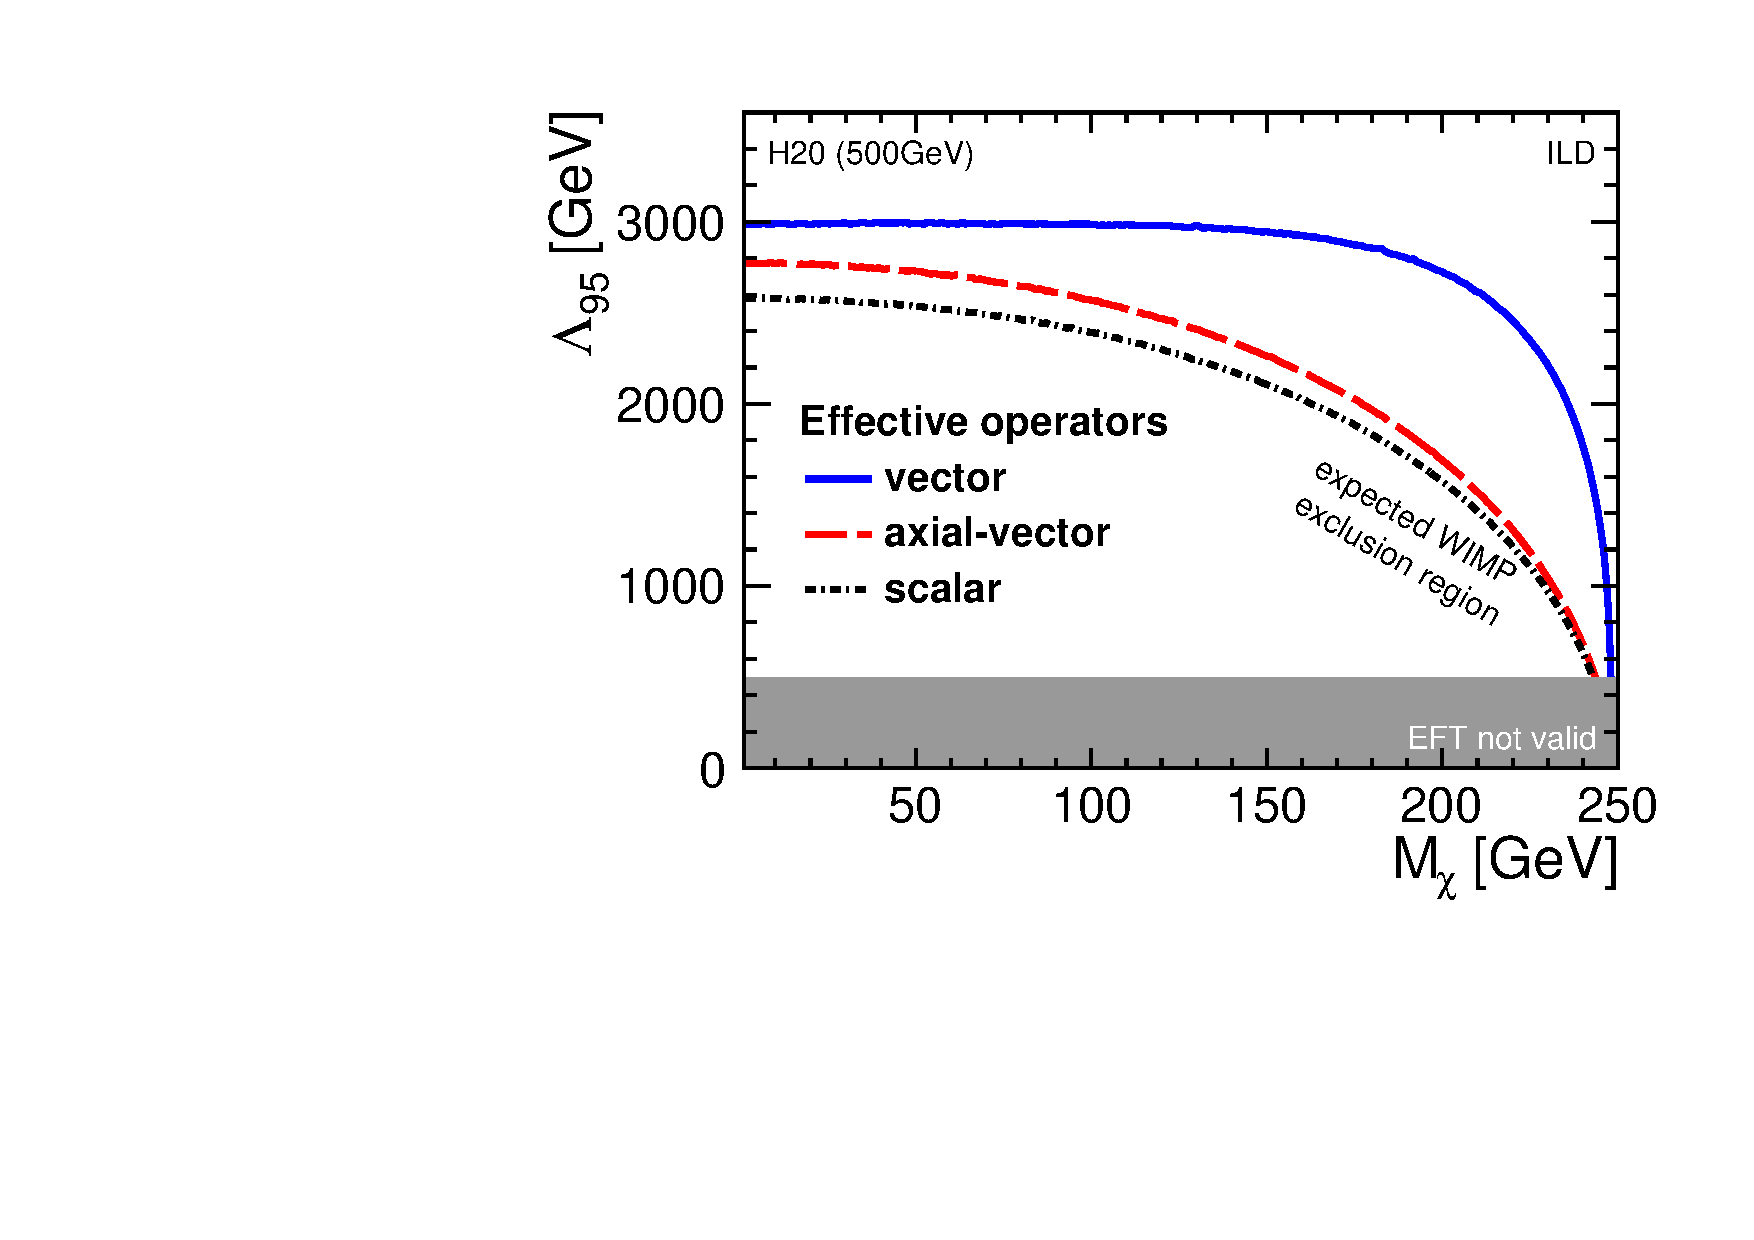
\includegraphics[width=0.45\linewidth]{chapters/figures/3operators_fullH20}}
\hspace{0.05cm}
\subfigure[]{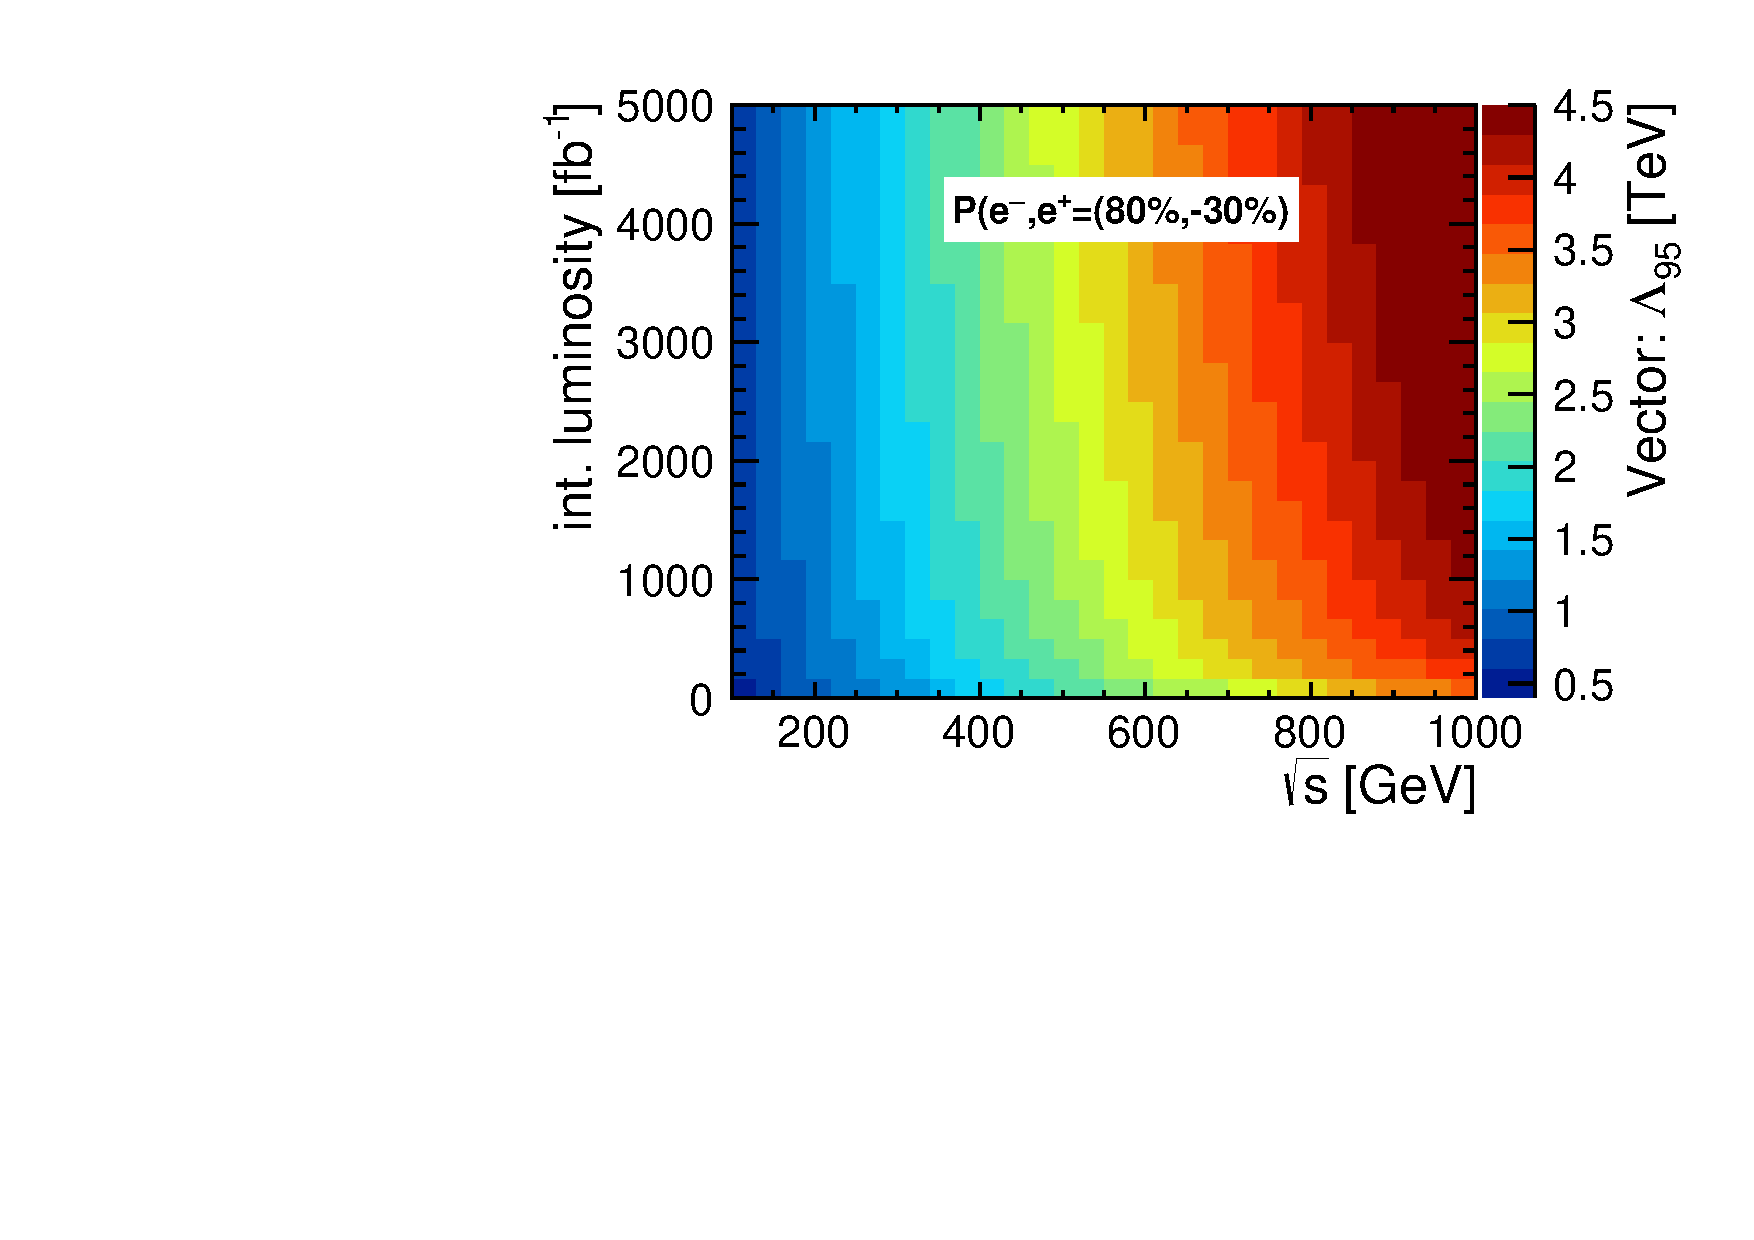
\includegraphics[width=0.45\linewidth]{chapters/figures/extrapolation_vector_pm}}
% \end{center}
\caption{\label{fig:searches_WIMPs} Left: Observational reach ($3\sigma$) of the ILC for a Spin-1 
  WIMP in terms of WIMP
  mass and $\kappa_e$ for three different chiralities of the WIMP-fermion couplings
%~\cite{bib:chaus}.
   Right: Expected sensitivity for a vector operator in an EFT-based interpretation as a function of integrated
  luminosity and centre-of-mass energy~\cite{Habermehl:417605}.}
\end{figure*}

\subsection{New scalars}
\label{subsec:searches_newscalars}

In many models with extended Higgs sectors, e.g.
Two Higgs Doublet Models, The Next-to-Minimal Supersymmetric  Standard  Model
and  Randall  Sundrum  models,  there  exists  a  light  scalar
$S^0$,
lighter than the Standard Model (SM) like Higgs.
The coupling of the $S^0$ to the $Z$ can be very small,
compared to the coupling a standard model Higgs with the
same mass would have
to the $Z$.
Such a light scalar with suppressed couplings to the Z boson would
have escaped detection at LEP.
With a factor of 1000 higher luminosity and polarised beams,
the ILC is expected to have substantial discovery potential for
this kind of states.
Furthermore,
searches for additional scalars at LEP and LHC are usually dependent on the
model details,
in particular on the decay branching ratios of the new scalar.
Thus, to be able to search for such new states,
it is paramount to have a more general analysis without
model-dependent assumptions.
The recoil-mass technique,
in particular with the Z boson decaying into a pair of leptons,
offers the possibility to achieve this.

The OPAL collaboration at LEP searched
for light scalars with this method,
but the  results were limited due to the low luminosity~\cite{Abbiendi:2002in}.
The luminosity offered by the ILC design being 1000
times higher than what LEP provided.
makes the recoil mass technique correspondingly more powerful~\cite{Asner:2013psa}
Therefore a search for a light scalar with a very weak interaction with
the Z boson using the model-independent analysis would become  viable
at the ILC-250.

A study was performed using the full Geant4-based simulation of the
ILD concept.
As a preliminary result~\cite{yanichep},
exclusion cross-section limits for
masses of the new scalar between 10 and 120
GeV are given in terms of a scale factor $k$ with respect to the
cross-section of the Standard Model Higgs-strahlung process would
have had, would the Higgs-mass have been the one assumed for the new scalar.

Background events are rejected by considering kinematic variables
only relied on muons. and the reconstructed $Z$:
The invariant mass, transverse momentum and polar angle of the muon pair,
as well as the polar angle of the missing momentum,
and the polar angle of each muon, and the angle between them.
Thus, no information on the decay of $S^0$ is used,
and the results will indeed be model-independent.
The recoil mass distributions obtained after applying the cuts
are shown in Figure~\ref{fig:searches_newscalars}a, 
for a number of hypotheses
on the mass of $S^0$, and $k=1$.
\begin{figure*}[]
\setlength{\unitlength}{1.0cm}
\subfigure[]{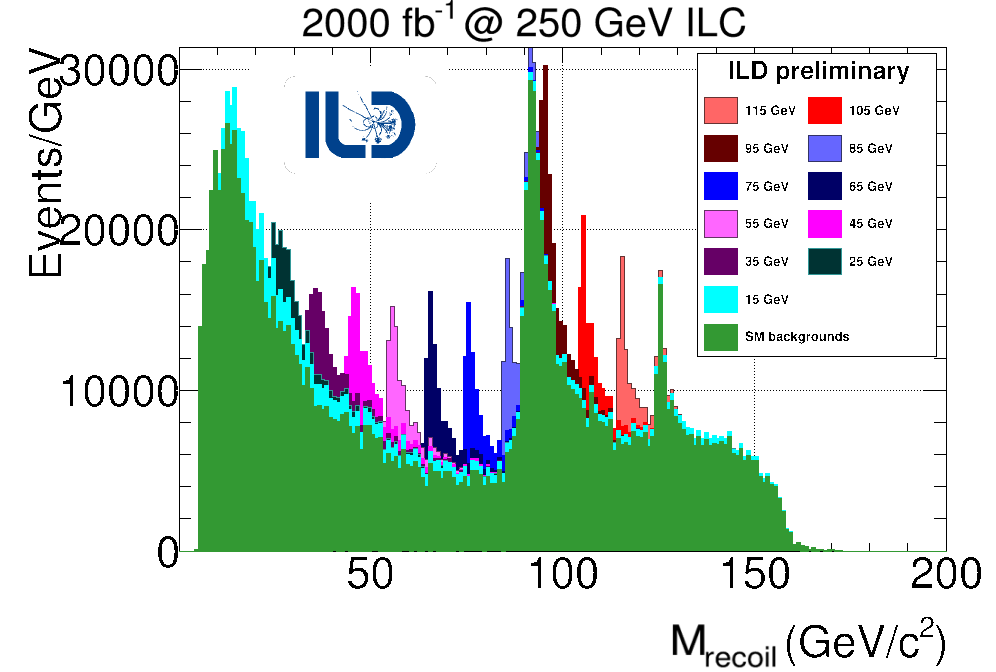
\includegraphics[width=0.45\linewidth]{chapters/figures/po_muon_kcut_recoil_mass_summary1}}
\hspace{0.05\linewidth}
\subfigure[]{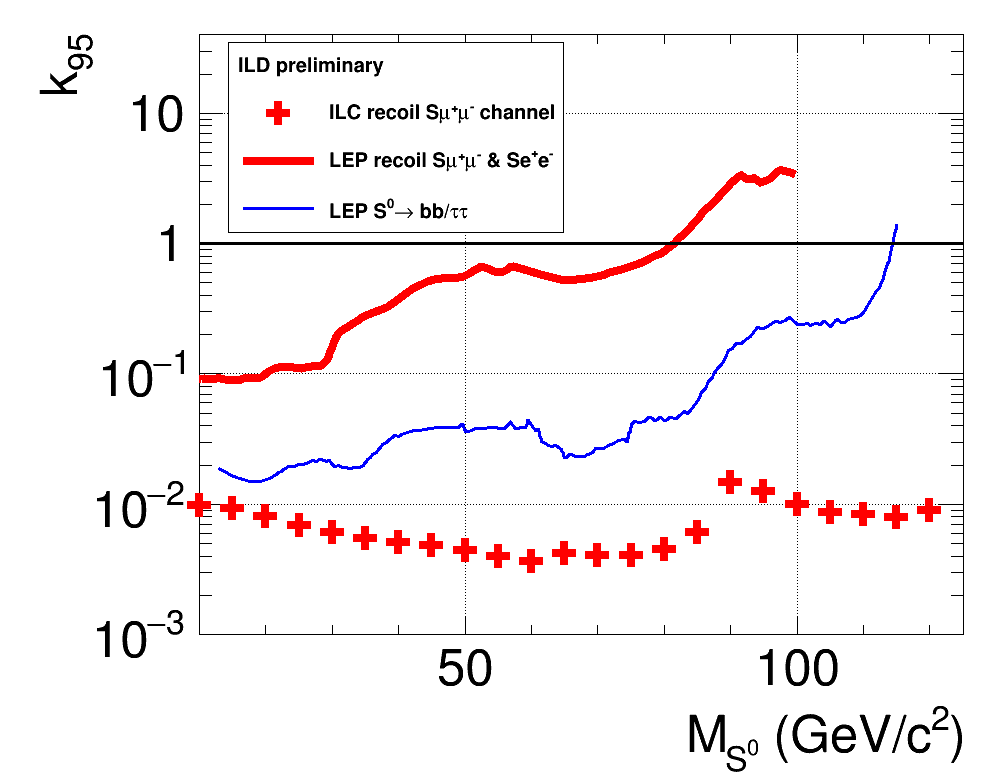
\includegraphics[width=0.45\linewidth]{chapters/figures/f_coupling_compare_LEP_and_PFO_final_cut_with_same_cut}}
% \end{center}
\caption{\label{fig:searches_newscalars} (a) The recoil mass distributions for various signals
and all backgrounds after the cuts.
(b) The 2 $\sigma$ exclusion limits for the cross section scale factor $k$ comparing the LEP and
ILC results. From \cite{yanichep}.}
\end{figure*}

The main backgrounds depend on the scalar mass.
In
the small mass region, the two fermions background
$\eeto \mu^+ \mu^-$ with an energetic ISR
photon is the overwhelming background;
while in the $Z$-pole region,
$\eeto ZZ \rightarrow \mu^+ \mu^- + X$
is an irreducible background,
as is - obviously - $\eeto Z^* \rightarrow ZH \rightarrow \mu^+\mu^- H$
at $M_{S^0} \sim M_H$.
The two fermion background can be
further rejected by taking into account ISR photon return effects.
The ISR photon veto cuts are applied to the ISR photons in the
centre region and forward region, separately.

The obtained 2 $\sigma$ expected exclusion limits for the
cross section scale factor
$k_{95}$ are shown for scalar mass from 10 \GeV to 120 \GeV
in  Figure~\ref{fig:searches_newscalars}b.
It is one to two orders of magnitude more sensitive than LEP, and
covering substantial new phase space.
In particular,
at all studied points, a new scalar with a a coupling to the $Z$ greater
than 1\% of that of a SM-higgs at the same mass would be excluded or
discovered at ILC-250.
